
\documentclass[english,12pt,a4paper,pdftex]{report}
%\documentclass[english,12pt,a4paper,dvips]{article}
\usepackage[sci]{aaltothesis}
\usepackage{graphicx}
\usepackage[colorlinks=true,urlcolor=red,linkcolor=black,citecolor=black,pdfstartview=FitH]{hyperref}

\usepackage{url}
\usepackage{amsmath}
\usepackage{algorithm2e}
\usepackage[toc,page]{appendix}
\usepackage{rotating}
\usepackage{color, colortbl}

\usepackage{array}
\usepackage{multirow}

\usepackage{amsfonts,amssymb,amsbsy}  

\usepackage{fancyvrb}


\setlength{\hoffset}{-1in}
\setlength{\oddsidemargin}{35mm}
\setlength{\evensidemargin}{25mm}
\setlength{\textwidth}{15cm}
\setlength{\voffset}{-1in}
\setlength{\headsep}{7mm}
\setlength{\headheight}{1em}
\setlength{\topmargin}{25mm-\headheight-\headsep}
\setlength{\textheight}{23cm}



% Colors
\definecolor{Good}{rgb}{0.44,1.00,0.25}
\definecolor{Neutral}{rgb}{0.42,0.85,0.18}
\definecolor{Bad}{rgb}{1.00,0.26,0.26}


\begin{document}

\department{Department of Mathematics and System Analysis}%
{Matematiikan ja systeemianalyysin laitos}
\professorship{Systems and Operations Research}{Systeemi- ja operaatiotutkimus}
\code{T3020}


\univdegree{MSc}
\author{Jussi Kolehmainen}

\thesistitle{Predicting Complex Events in Sensor Data}{Monimutkaisten tapahtumien ennustaminen sensoridatasta}

\place{Espoo}
\date{08.08.2013}

\supervisor{Prof.\ Ahti Salo}{Prof.\ Ahti Salo}
\instructor{M.Sc.\ (Tech.) Antti Aalto}{DI Antti Aalto}

\uselogo{aaltoRed}{''}

\makecoverpage



\keywords{monimutkaisten tapahtumien prosessointi, ennustaminen, ymp\"arist\"odata, taloautomaatio, tukivektorikoneet, wavelet-analyysi}
%% Tiivistelm�n tekstiosa
\begin{abstractpage}[finnish]
Monimutkaisten tapahtumien prosessointi (CEP) on teknologia, joka analysoi datavirtoja ja tunnistaa monimutkaisia tilanteita reaaliajassa. Tunnistettavat tilanteet m\"a\"aritell\"a\"an EPL-lauseilla, joiden kirjoittamiseen tarvitaan tutkittavaa ilmi\"ot\"a tuntevia asiantuntijoita. Yhdess\"a matemaattisten ennustemenetelmien kanssa CEP mahdollistaa tapahtumien ennustamisen ja niist\"a varoittamisen.
\\ 
\\
T\"ass\"a ty\"oss\"a k\"ayn l\"api mit\"a ennustava tapahtumaprosessointi on ja kuinka eri komponenteista voidaan kasata j\"arjestelm\"a reaalimaailman tapahtumien ennustamiseen. Matemaattisina ty\"okaluina k\"ayt\"an kahta mallia: et\"aisyysmittaan perustuvaa mallia ja piirrevektoriin perustuvaa mallia. Ensimm\"ainen k\"aytt\"a\"a DTW:t\"a et\"aisyysmittana ja k:n l\"ahimm\"an naapurin (kNN) algoritmia luokitteluun. J\"alkimm\"ainen pohjautuu wavelet-analysiin ja tukivektorikoneisiin (SVM).
\\
\\
Kokeellisess\"a osiossa esittelen taloautomaation sovellutuksena ennustavalle tapahtumaprosessoinnille. Testeiss\"a k\"ayt\"an todellisia sensoreita, joille ennustan sis\"ailmayhdistyksen asettamien raja-arvojen ylityksi\"a. T\"am\"an lis\"aksi arvioin rakentamani systeemin suorituskyky\"a.
\\
\\
Hiilidioksidille ja haihtuville orgaanisille yhdisteille ensimm\"ainen malli antaa oikeita h\"alytyksi\"a yli 75 \%:ssa tapauksista ja p\"a\"asee alle 10 \%:iin v\"a\"arien h\"alytysten osalta. J\"alkimm\"ainen malli toimii nopeammin, mutta sen konfigurointi osoittautuu haastavaksi, mink\"a takia tulokset ovat huonompia. Jatkotutkimusten aiheiksi suosittelen erityisesti j\"arkev\"amp\"a\"a tapahtumam\"a\"arittely\"a ja systeemin aikaparametrien parempaa optimointia.
\end{abstractpage}

\newpage

\keywords{complex event processing, predictive analytics, environmental data, house automation, support vector machines, wavelet analysis}
%% Abstract text
\begin{abstractpage}[english]
Complex event processing (CEP) analyzes data streams and detects complicated situations in real-time. Domain experts write effective EPL (event processing language) queries to define complex events that are detected. In combination with predictive analytics (PA), which uses mathematical models to predict the future, a framework for predicting complex events can be designed.
\\
\\
In this thesis I describe how predictive event processing works and how a proof-of-concept framework can be built. As prediction tools I use two models: a distance-based model and a feature-based model. The former uses dynamic time warping (DTW) and k-nearest neighbour (kNN) algorithm while the latter employs wavelet analysis and support vector machines (SVMs).
\\
\\
As an application of predictive complex event processing I consider house automation and present a real-life case study for the experimental section. The goal is to predict when a certain variable exceeds a limit value for a certain period of time. I also evaluate the performance of the system.
\\
\\
With two variables, $\mathrm{CO}_2$ and VOC (volatile organic compounds), the first, distance-based model performs better with correct alarm rate of over 75 \% and false alarm rate of under 10 \%. The second, feature-based model turns out to be faster but more difficult to configure properly. More meaningful complex events and more thorough time parameter optimization are suggested for future research.





\end{abstractpage}

\mysection{Acknowledgements}
%\mysection{Preface}
First, I want to express my deepest gratitude towards my family who has always supported and encoraged me in my studies. You have helped me to achieve yet another goal in my life. Second, I want to thank my supervisor, Ahti Salo, and my instructor, Antti Aalto, for guiding me through the writing process. Third, I want to thank my employer HiQ Finland and especially Jukka-Petri Sahlberg for permitting me to write this thesis for the MMEA research program. I also want to thank the research group of environmental informatics at the University of Eastern Finland and especially Mauno R\"onkk\"o for giving me access to their test data. All in all, thanks to everyone who supported me and helped me through this long but rewarding process.
\\
\\
Albert Einstein once said: \emph{"Once we accept our limits, we go beyond them"}. This thesis used to be one of them. Now I have to accept that my limits have once again moved a big step further.


\vspace{5cm}
Otaniemi, 08.08.2013

\vspace{5mm}
{\hfill Jussi Kolehmainen \hspace{1cm}}


\newpage
%

\addcontentsline{toc}{section}{Contents}
\tableofcontents

\mysection{Symbols and abbreviations}
\subsection*{Symbols}

\begin{tabular}{ll}
%$|a_{ij}|^2$, $|a_i|^2$ & probability of two electrons having momenta
%    $\boldsymbol p_i$ and $\boldsymbol p_j$ ($\boldsymbol p_i$ for $|a_i|^2$) \\
%                 & at any given instant \\
$\mathbf{AC_d}$ & ROC distance from optimal classifier \\
\textbf{C} & SVM soft margin parameter \\
$\mathbf{\gamma}$ & SVM kernel parameter \\
\textbf{k} & kNN parameter \\
\textbf{radius} & DTW warping path parameter \\
\end{tabular}

%\subsection*{Operators}

%\begin{tabular}{ll}
%$x$ & example
%\end{tabular}

\subsection*{Abbreviations}

\begin{tabular}{ll}
\textbf{DTW} & Dynamic Time Warping \\
\textbf{DWT} & Discrete Wavelet Transform \\
\textbf{EPA} & Event Processing Agent \\
\textbf{EPN} & Complex Event Network \\
\textbf{CEP} & Complex Event Processing \\
\textbf{kNN} & k-Nearest Neighbor \\
\textbf{PEPN} & Predictive Event Processing Network \\
\textbf{ROC} & Receiving Operator Characteristics \\
\textbf{SVM} & Support Vector Machine \\
\\
\textbf{P} & Positives, number positive instances \\
\textbf{N} & Negatives, number of negative instances  \\
\textbf{TP} & True Positives \\
\textbf{FP} & False Positives \\
\textbf{TN} & True Negatives \\
\textbf{FN} & False Negatives \\
\textbf{TPR} & True Positive Rate \\
\textbf{FPR} & False Positive Rate \\
\textbf{TNR} & True Negative Rate \\
\textbf{FNR} & False Negative Rate
\end{tabular}


\cleardoublepage
\storeinipagenumber
\pagenumbering{arabic}
\setcounter{page}{1}


\chapter{Introduction}
\section{Background}
As the size of the digital universe, that is, the total size of digital data in the world is approaching zettabytes (trillion gigabytes) \cite{IDC},  more and more ways are needed to make sense of that information. One of the biggest technology trends in this decade, big data refers to the analysis of large volumes of data. The definition of the term big data varies a lot but some common characteristics can usually be found: conventional database systems are not enough because the data is too big, moves too fast or does not fit in the current data structures. \cite{Dumbill12}

Complex event processing (CEP) can be thought as a branch of big data in which the speed of the data flow is too much for the ordinary databases to handle. CEP tackles this issue by providing event-driven processing, for example pattern detection and causality analysis, with extremely low latencies. \cite{CEP10} It reverses the idea of conventional databases: instead of running queries against an existing data set, CEP uses predefined queries against which the data is run.

Despite these evident advantages of CEP in real-time data processing, it is only a technological opportunity without domain expertise. Like a database expert writes complex SQL queries that return the desired dataset, a CEP expert writes EPL queries that filter the data flow in some way. However, it is possible to reduce the amount of human work needed by extending a CEP engine with other advanced technologies, such as machine learning (ML) and predictive analytics (PA). \cite{Fulop12} In this thesis, I will present a framework for predictive complex event processing (PCEP) that is capable of predicting an event beforehand by learning the pattern that precedes the event.

A promising field of application for complex event processing is ambient intelligence, or house automation, which comprises smart homes that are able to change the living environment depending on various indicators. \cite{Augusto04} Smart homes gather information, for instance, about the whereabouts of the people living in them, air quality and electricity consumption. From these factors the smart homes can then adjust heating, ventilation and lights accordingly. CEP can provide an efficient platform for this real-time data gathering and analysis. This thesis contains a real-world study case from the field of house automation. By combining complex event processing, predictive analytics, and sensor data, smart homes can be made to think one step ahead.

The learning and prediction phase are implemented with relatively new techniques, namely Wavelet Analysis and Support Vector Machines (SVMs). While Fourier Transform captures only the frequency domain properties of a signal, wavelets are localized in both time and frequency domains. \cite{Fong04} Thus, wavelets can be used to extract informative patterns from sensor data. These patterns, then, are classified with  binary classifiers, SVMs, into patterns that precede certain events and patterns that do not.

As a comparative method a k-Nearest Neighbor algorithm in combination with Dynamic Time Warping (DTW) measure is used. DTW is an extension of Euclidean Distance and it is more suitable for comparing time series.

This thesis is part of a five-year research program called The Measurement, Monitoring and Environmental Assessment (MMEA). The program aims at creating new tools for environmental data usage in both consumer and industry sector. The environmental data available from sensor data producers will be made available to data consumers in an open-source marketplace where the parties can connect with their own software. \cite{MMEA}


\section{Motivation for Predictive Event Processing}
A system that is capable of predicting events instead of just detecting them can prevent undesirable conditions from happening. An apparent field of application where these undesirable conditions might be harmful for humans is house automation. Moreover, a system like this can save energy by adjusting control variables more efficiently and provide the residents automated changes of the living conditions. \cite{Skon}

A good example of harmful living conditions is the rise in the concentration of carbon monoxide, which is a highly toxic gas. Being completely colorless, odorless and tasteless, it can only be detected with specific sensors. However, detecting the risen concentration is not enough as the poisonous gas is already present and the residents are in danger. By detecting the increase the house could alert the residents and set the ventilation to full-speed. \cite{Yeganeh12} Another example of harmful situation that could be avoided with a predictive system is flood. The rise in the water level that leads to a flood must be distinguished from the normal seasonal variation. \cite{Verbunt07} 

An intelligent control of heating, especially floor heating, can create significant energy savings because of the long delay between controlling the heating settings and the actual heating effects. In a classical heating system, such as a radiator, the delay does not need to be taken into account because it reacts to the control in minutes and emits its energy to the surroundings. An intelligent floor heating, however, requires predicting the future energy prices and outside temperatures, because the floor should be heated during off-peak hours when the prices are lower or when outside temperatures are about to fall. \cite{Chen11}

Comfortable living conditions are not achieved by merely avoiding harmful conditions. A constant temperature, which increases living convenience remarkably, cannot be maintained if the heating system does not adapt to substantial changes in outside temperature beforehand. Also the concentration of volatile organic compounds (VOC), which is one of the test cases in this thesis, should be kept as low as possible in order to maintain good air quality. Again, a predictive component with machine learning algorithms is needed to adjust the ventilation before the concentration hits a critical level. The system should also adapt to the residents' lifestyle and schedule the changes in indoor air conditions accordingly. \cite{Skon}


In addition to house automation, predictive event processing can be used in such fields as financial markets and traffic control. As the stock market is nowadays mostly run by automated algorithms, the speed of data processing is a critical factor. Combined with predictive machine learning components, such system could attain crucial advantage against its competitors. Traffic control system, in turn, could predict traffic jams from past data. By varying speed limits and guiding vehicles to less occupied roads, it could reduce emissions and travel times. \cite{Bellemans06}


\section{Research Questions and The Scope of This Thesis}
Complex Event Processing (CEP) is mostly used for detecting known patterns in the data stream. When CEP is used to analyze our surrounding world, it is relatively easy to detect a certain situation that can be undesirable for humans, animals or some materials. However, the actions to prevent those conditions from happening should usually be taken long before that as it was mentioned in the previous section.

The main research question of this thesis is to formulate a framework for combining CEP and Predictive Analytics (PA). There is plenty of research done from both areas but not many papers have dealt with combining them. The most important inspiration for this thesis is the work done by Hungarian scientist Lajos Jeno F\"ul\"op and his colleagues at Nokia Siemens Network. They tried to detect and predict the number of persons entering and leaving a building. Their application employed decision tree algorithms, such as BFTree, for detecting conditions that precede a traffic peak. \cite{Fulop12}

One of the novel topics in this thesis is the data handling with CEP. The framework not only detects the complex events with CEP but also creates sliding windows for collecting the data training and labeling it into positive and negative samples. The goal of this approach is to test the capabilities of CEP for more than just its main purpose, detection of events that have already been occurred.

The two models used in this thesis were chosen by suggestions from research papers and literature. The first model, which uses DTW and kNN, is a very simple approach for time series classification. DTW has been used in many research applications and has been proven to achieve one of the smallest error rates with many data sets (e.g. \cite{keogh05}).

The combination of Wavelets and SVMs were chosen as our second model because it represents a much more modern approach. Even though Haar Wavelets were first discovered in the early 1900s, the theory of Wavelets has been evolving still in the 2000s in the form of image compression and trend detection \cite{waisberg11}. The Support Vector Machines (SVMs) were first mentioned in 1979, but formally introduced by Vladimig N. Vapnik as late as in 1995 \cite{bosswell02}.

In the light of past results with DTW and SVM based classification it would be a big surprise if the latter would achieve better performance. \cite{keogh05} \cite{Hautakangas11} The main reason for this is that tuning of both Wavelets and SVMs is much more challenging task than using simple DTW and kNN based model which has only two parameters.




\section{Structure of This Thesis}
Chapters 2.1 and 2.2 present the principles of complex event processing (CEP). Chapter 2.3 introduces a CEP Engine called Esper which is used in the experimental part of this thesis. The Event Processing Language (EPL) for Esper is also reviewed. Chapter 2.4 briefly reviews some applications of CEP.

Chapter 3.1 defines predictive analytics (PA) and Chapter 3.2 discusses how it can be integrated with CEP. Chapter 3.3 formulates the problem for time series prediction. Chapters 3.4 and 3.5 present mathematical models for time series prediction. The former focuses on distance based methods while the latter describes what feature based classification is. Chapter 3.6 shows how the performance of these methods can be evaluated.

Chapter 4 begins with introducing the case study and the available test data. Then, Chapter 4.2 continues with describing the implementation of a Predictive Event Processing Network (PEPN). Chapter 4.3 briefly reviews the MMEA platform architecture and explains how the predictive component could be integrated. Chapter 4.4 defines the complex events we are trying to predict and presents methods for parameter tuning.

Chapter 5 presents the performance results of the classifiers. Then, it discusses computational performance.

Chapter 6 sums up the results of this thesis and discusses further research possibilities from the field of predictive complex event processing.




\clearpage

\chapter{Complex Event Processing}
\section{Events and Patterns}
One definition for an event is ``anything that happens, or is contemplated as happening''. \cite{Luckham08} According to this wide definition, there is a huge number of events occurring around us all the time. Examples of these events include opening a door, receiving a measurement value from a sensor and the ending of the World War II. It can easily be seen that we need to further classify events in order to be able to define a system for event processing.

Events can be divided into two groups: simple and complex events. \cite{IBM10} A simple event is any single instance that comes into our system from sensors. Thus, a simple event is a single measurement value. Complex events, on the other hand, are derived from the single events and are something that we want to detect from the event stream. They are the result of the event processing system. Examples of complex events that we are interested in thesis are a single measurement variable rising at a certain speed and a group of variables exceeding a threshold value for a certain amount of time.

An event sequence is ``a time-ordered sequence of events''. \cite{Weiss98} For example, a series of consecutive measurement values form an event sequence. An event pattern is an event sequence with given values for the events. \cite{Luckham08} Hence, a peak and a rise in a variable are both event sequences but are classified as different event patterns. In this thesis I assume that the complex events of our interest can be predicted by detecting the event pattern that precedes the event. 



\section{Overview of a General Event Processing System}
An outline of a complex event processing system is presented in Figure~\ref{fig:event_processing_network}. The inputs of the network are the event sources that produce simple events. They can be, for instance, thermometers or movement sensors. An Event Processing Agent (EPA) is a node in the network that consumes events, performs some predefined tasks, and produces new events based on its rules and input events. Possible tasks for an EPA include event filtering, aggregating and pattern detection. \cite{Fulop12}

\begin{figure}[here]
\centering
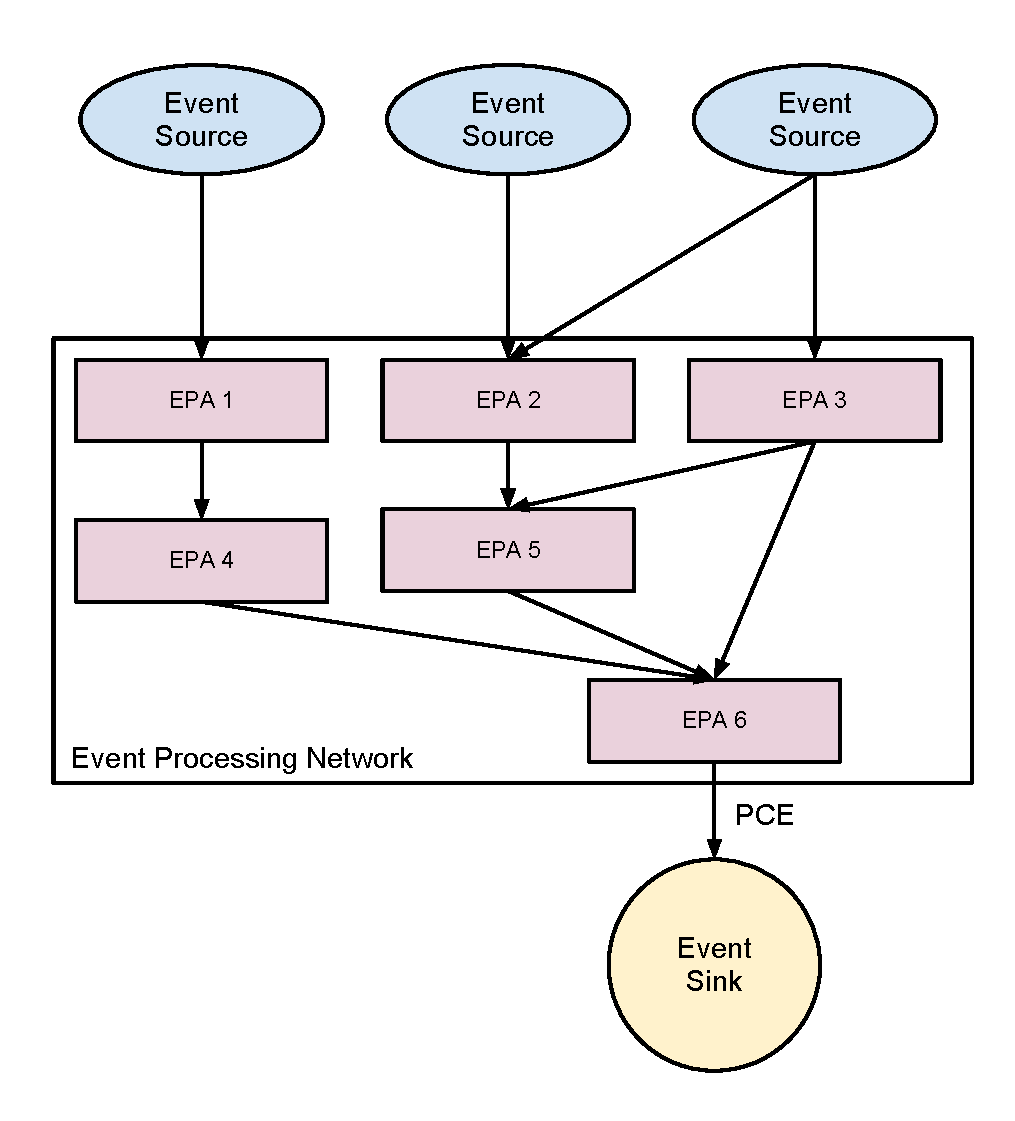
\includegraphics[scale=0.7]{images/event_processing_system.pdf}
\caption{Event Processing Network.}
\label{fig:event_processing_network}
\end{figure}

All the nodes in the network are connected via event channels (arrows in the figure). It is suggested that at this point the event channels are high-level abstractions and we do not limit the types they can handle nor the number of sources or consumers attached to them. \cite{IBM10}

A group of interconnected EPAs form an Event Processing Network (EPN). An EPN has the following properties: it can by dynamic (EPAs can be created and destroyed), it may contain feedback loops and it can be distributed across multiple physical computers. \cite{Luckham08} However, in the study case of this thesis we do not need any of those properties because the complex events we are interested in are rather simple ones.

As a result, an EPN produces a Primary Complex Event (PCE) that goes to the event sink. A PCE has the prefix primary in order to distinguish it from the complex events passed between EPAs. A PCE is the event whose future occurrences we are trying to predict in this thesis. The event sink represents all the parties who are interested in the complex event in question, including both automated machines that are triggered to perform some action and human workers who are notified when something interesting happens. \cite{Fulop12}


\section{CEP Engines and Processing Languages}
There is a wide range of Complex Event Processing Engines with different properties available on the market. First started in the Bell Labs in the mid 90's, the CEP business sector has spanned into more than 20 widely used products from all the major IT houses, such as IBM, Microsoft and Oracle. \cite{Vincent11}  

CEP engines can be divided into four subcategories based on abstraction type for event detection and action triggering. In the first category, Data Stream Query Languages, a SQL-like language is used to create relational queries against the data stream. In the second category, Production Rule Languages, queries are based on a set of condition-action pairs stored in the working memory. When a condition becomes true, the corresponding actions is fired. In the third category, Composition-Operator-Based Languages, operators are used to define complex causal queries based on simple queries, such as whether or not a certain event happens. The last category is rarer; the languages in it use logical XML formulas for automated reasoning in a Semantic Web. \cite{Bui08}

Most CEP engines have several common features that are used to handle the data stream. As all the events in CEP are somehow typed, filtering can be used to select only the ones that we are interested in. Windows, specified either with time interval or a number of events, allow us to use a subset of the stream for processing. Data aggregation, conjunctions and disjunctions can be used to create more abstract levels of events. Temporal and causal relationships between events are efficient in reasoning complex sequences and patterns of events. Of course, negation and counting methods are available for detecting the presence or absence of events. \cite{Marcelo09}

In MMEA program, and consequently in this thesis, we use an open-source, Java-based CEP engine called Esper. Esper has properties from the first three categories listed above. It uses Event Processing Language (EPL) to specify expressions for pattern matching and for detecting the presence or absence of events \cite{EsperReference}. A standard EPL query is of the form

\begin{Verbatim}[xleftmargin=1.5em]
INSERT INTO
	[stream]
SELECT
	[attributes]
FROM
	[stream]
WHERE
	[condition]
GROUP BY
	[attribute]
HAVING
	[condition]
\end{Verbatim}

The \emph{SELECT} clause is used to select which attributes we want to catch from each event that matches our filter. The optional \emph{INSERT INTO} clause puts these attributes into a new stream. The \emph{FROM} clause specifies the streams and corresponding time windows we are looking into. The \emph{WHERE} clause can filter the events, for example, by giving a threshold value for a certain event attribute. The \emph{GROUP BY} clause is used to aggregate several events of the same type into an abstraction event, for instance, by event type. The \emph{HAVING} clause is used filter the aggregated events formed by \emph{GROUP BY}. \cite{Bui08} 

In Esper, Events can be POJOs (Plain Old Java Objects), Maps (key-value-dictionaries) or XML documents. All event types have attributes that can further have sub-attributes of any type. \cite{EsperReference} In the following, I will present some examples of Java POJOs in Esper.

Say we have the following Java class
\begin{Verbatim}[xleftmargin=1.5em]
public class Sensor {
	int id;
	String name;
	Sensor[] groupSensors;  
}
\end{Verbatim}

A Sensor has an identification number, name and a list of other sensor belonging to the same group. Furthermore, say we have an event type called \emph{SensorEvent} which represents a single measurement that comes from a sensor:
\begin{Verbatim}[xleftmargin=1.5em]
public class SensorEvent {
	Sensor sensor;
	Timestamp timestamp;
	Map<String, Double> measurements;
}
\end{Verbatim}

A \emph{SensorEvent} has a reference to the sensor from which the event originated, a timestamp that captures the exact point in time when the measurement was made and a map that contains key-value pairs where the key is the variable name (e.g. temperature) and the value is the measurement value (e.g. 10.9 degrees celsius).

Now we can refer to the event attributes in an EPL query in the following way:

\begin{description}
	\item[Simple: SensorEvent.timestamp] \hfill \\
	measurement time
	\item[Nested: SensorEvent.sensor.id] \hfill \\
	sensor id
	\item[Indexed: SensorEvent.sensor.groupSensors{[0]}.name] \hfill \\
	name of the first sensor in the same group
	\item[Mapped: SensorEvent.measurements('temperature')] \hfill \\
	value of the temperature measurement
\end{description}

Next, I will present some examples of the query types we might need in the study case of this thesis. To select the name of the sensors that have the temperature exceeding 20.0 degrees can be done using the following query:

\begin{Verbatim}[xleftmargin=1.5em]
SELECT 
	sensor.name 
FROM 
	SensorEvent 
WHERE 
	measurements('temperature') > 20.0
\end{Verbatim}

To retrieve the average humidity from each sensor every 30 minutes we can use a timed window:
\begin{Verbatim}[xleftmargin=1.5em]
SELECT 
	avg(measurements('humidity')) 
FROM 
	SensorEvent.win:time_batch(30 min) 
GROUP BY 
	sensor.id
\end{Verbatim}

To define a sliding window of 30 minutes that is triggered on every new instance, we can change the \emph{win:time\_batch} to just \emph{win:time}. A time interval can be defined with \emph{timer:interval}. Combined with the patterns described below, it is useful, for example, when a certain event has to happen within 10 minutes of another event.


As an example of event pattern detection, let's assume we have a stream (called Stream) of events: $A_1 \ A_2 \ B_1$. This example was originally shown in Esper Reference \cite{EsperReference}. Now the pattern

\begin{Verbatim}[xleftmargin=1.5em]
SELECT 
	every a=A -> b=B 
FROM 
	Stream
\end{Verbatim}
matches each A followed by B ([$A_1 \ B_1$], [$A_2 \ B_1$]) but the pattern

\begin{Verbatim}[xleftmargin=1.5em]
SELECT 
	every a=A -> (b=B and not A) 
FROM
	Stream
\end{Verbatim}

matches every A followed by B but not A. In this case, the resulting event is only [$A_2 \ B_1$].


As one can see, by combining windows, relational clauses and SQL-like procedures, such as sub-queries and joins, we are able to define quite complex queries that would be hard to implement in conventional programming methods. This thesis does not focus much on the writing of effective EPL queries for detecting complex events, but rather assumes that the queries have already been defined by some domain expert. 

By default, Esper uses system's time when creating windows and handling causality. This behavior can be bypassed by turning Esper's internal clock off and constantly sending \emph{CurrentTimeEvent} objects into the engine with a selected timestamp. \cite{EsperReference} 


\section{Applications of CEP}
Complex event processing (CEP) has found applications in many fields from Business Process Monitoring (BPM) to intrusion detection in computer networks. In this chapter I present some successful examples of using CEP for high-speed data processing.

Radio frequency identification (RFID) is a technology for identifying physical objects by equipping them with a remote-readable tags that can be read using radio-frequency electromagnetic fields. Then, the lifespan of the object can be monitored more accurately than with any other method. In big industrial companies this produces a huge amount of data that has to processed and analyzed in real-time in order to get the maximum benefit from the RFID technology. CEP provides a great platform for filtering the RFID data, aggregating semantic information into the data and routing the data to customers and suppliers. \cite{Wang06}  

In the financial sector, where tremendous amounts of data are passed between banks and customers constantly, it is no surprise that the data can be transferred and processed effectively with CEP. Example use cases are detecting suspicious money transfers and credit card frauds by monitoring where the credit card has been used and how much money has been withdrawn with it. In stock market CEP can be used to follow market trends and correlations between different stocks. \cite{Adi06}

Business process management (BPM) and CEP can be integrated to provide valuable information to customer relationship management (CRM). By monitoring real-time customer interactions, such as clicks in an e-commerce or comments on a blog, business providers can create automated actions that personalize service to each customer. Event-driven actions can even indicate the customer's emotional state, which may be used for targeted advertising. \cite{Kobielus08}

In combination with predictive analytics (PA), which we will discuss more in chapter 3, CEP can be utilized to detect and locate failures in component based systems by online tracking. Chen et al. \cite{Chen06} monitored the distribution between signal and noise subspaces, and detected failures with online distribution learning algorithms. 


\clearpage

\chapter{Predictive Analytics}
\section{General}
Predictive analytics (PA) is a broad field of applied mathematics. First, it includes all the statistical models and empirical methods that are used to create empirical predictions. Second, also predictive power, that is, methods for assessing the quality of predictions is a part of PA. \cite{Shmueli10} Another purpose of PA is to guide theory building, theory testing and relevance assessment. \cite{Dubin69}

One way to classify PA methods is to divide them into predictive models, descriptive models and decision models. Predictive models look for the most significant explanatory variables with which they are able to predict the dependent variables. Descriptive models, in turn, try to find as many relationships as possible, leading to segmented models that describe the world as it is. Decision models use optimization techniques to find the most optimal decision based on possible outcomes. \cite{Fico06}

Another way to classify PA methods is to distinguish between methods that predict the present and methods that shape the future. Predicting the present means applying patterns of current behavior with as much historic data as possible. These methods use classification, regression, clustering and all data mining techniques to predict similar occurrences in the future. Shaping the future has to do with generating new standards after the underlying assumptions have changed. While predicting the present can be thought as fitting a curve into the existing data, shaping the future creates a totally new curve with new assumptions and anticipated behaviors. \cite{Oracle10} In this thesis, all the used methods can be classified as predicting the present.

The methods of PA can also be divided into regression and machine learning  techniques. The simplest model is probably linear regression, which tries to find a linear model between a set of independent variables and a dependent variable by minimizing the squared error \cite{Montgomery12}. Time series models assume that the process we are investigating has some kind of internal structure with autocorrelation, trend or seasonal variation. This structure may be discovered with either time-domain or frequency-domain analysis. \cite{Hamilton94} The former is based on auto-correlation and cross-correlation analysis, while the latter is carried out with spectral or wavelet analysis, which I will talk about more in chapter 3.5.

Machine learning algorithms form a model, based on clustering or historic data, that is able to predict the class of the dependent value without necessarily knowing the exact mathematical structure behind it. As an example of clustering based methods, unsupervised Artificial Neural Networks (ANNs) are biology-inspired complex networks that evolve into a form that can classify new instances into a group with the most similar instances. \cite{Mitchell97} Models based on historic data are called supervised models and they can, for example, find a classifier function that separates the training data most effectively. I will talk more about classifiers in chapter 3.5 when I introduce Support Vector Machines.



\section{Combining CEP and PA}

The work of Fulop et al. \cite{Fulop12} lists several synergies and differences of CEP and PA which are briefly summarized in this section. 

Complex event processing (CEP) and Predictive Analytics (PA) are similar in the sense that they try to somehow make sense of large datasets, either in real-time or from historic data. The biggest differences between CEP and PA stem from the timing of the reasoning process. While CEP processes data real-time and detects the events only after they have occurred, PA, as the name suggests, tries to predict events by detecting the patterns that lead to them. 

\begin{figure}[here]
\centering
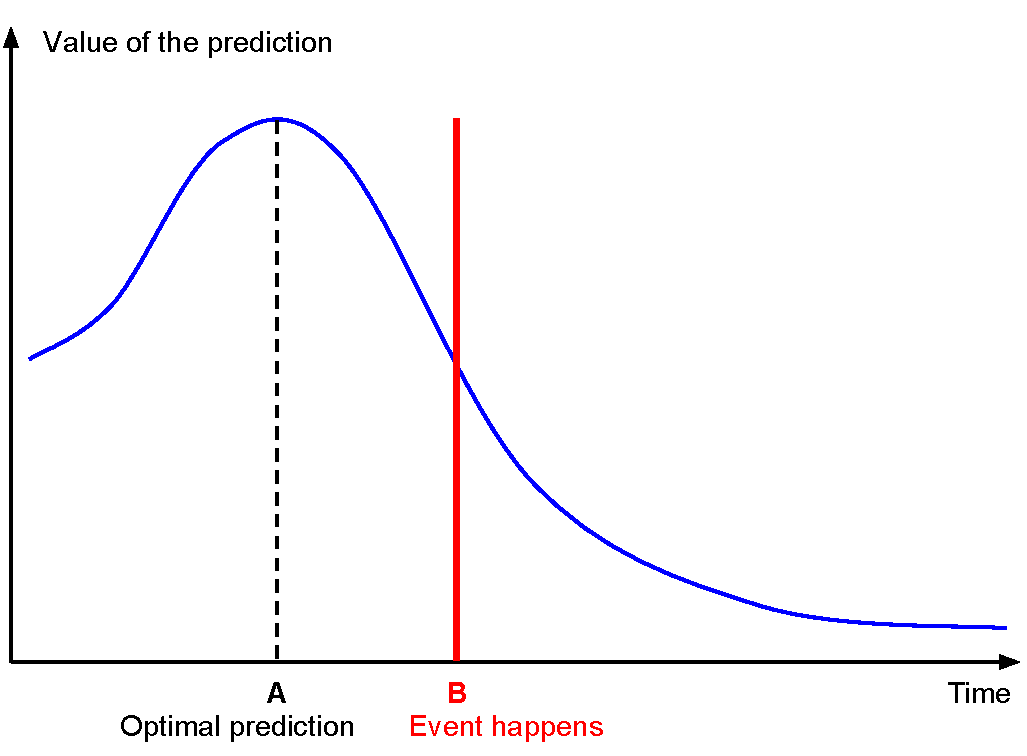
\includegraphics[scale=0.7]{images/prediction_value_v2.pdf}
\caption{Expected value of event detection as a function of time. An optimal prediction is made at the point A. The event happens at the point B, after which detecting the event is still valuable.}
\label{fig:prediction_value}
\end{figure}

The (expected) value of detecting an event depends directly on time, which is illustrated in Figure~\ref{fig:prediction_value}. Up to point A, value increases with increased accuracy. This is because long time predictions are not usually accurate. Nevertheless, since an early prediction is more useful than one that is made just a few seconds before, the value begins to fall rapidly. After the point B where the event actually happens, detecting an event is still useful and the value decreases slowly. The optimal prediction point A in Figure~\ref{fig:prediction_value} motivates this thesis' search for a predictive event processing model.

Another difference between CEP and PA is the need for building rules that detect patterns. CEP relies heavily on predefined rules that have to be implemented by a domain expert that knows the complex event in question. This can be considered a weak point of CEP. PA, in turn, aims at automating the rule creation. Of course, PA methods need to be implement, too, but that happens before the model is crafted into a certain scenario. The model should then adapt to different kinds of scenarios. In CEP a specialized model is required for each different scenario.

There are several requirements that should be taken into consideration when designing a predictive CEP system. First, CEP and PA components must be able to communicate with each other so that CEP receives Primary Complex Event (PCE) predictions from PA and PA receives predictors from CEP. Second, integrating the PA component should not affect the existing CEP part nor its maintainability in any way. \cite{Fulop12}

There are two ways to overcome these requirements. The first is to introduce predictive event processing agents (PEPAs) into the Event Processing Network (EPN). The second is to create a separate predictive event processing network (PEPN) that is somehow connected to the original EPN. Only the latter of these options satisfied the condition that the original EPN should not be affected in any way. The maintainability of EPN suffers greatly if PEPAs are mixed with original EPAs. \cite{Fulop12} The implementation chapter describes how this requirement is actually fulfilled. 


\section{Predicting with Time Series Classification}
Our task is to predict whether or not a certain event will happen in a defined time period in the future. Figure~\ref{fig:prediction_time_span} shows an outline of this process. Let's assume that the complex event we are trying to predict occurs between $t_{E,1}$ and $t_{E,2}$. Then, in order to gain advantage from predictive analytics, the prediction should happen before the warning time begins at $t_{P,2}$. We can define a prediction time period to be the interval from $t_{P,1}$ to $t_{P,2}$, which contains the event history available for making the prediction. Thus, we can assume that the prediction happens at $t_{P,2}$ and uses information from $t_{P,1}$ to $t_{P,2}$. In Chapter 4 I will discuss how to choose the interval lengths 

\begin{eqnarray}
\textbf{windowLength} &=& t_{P,2} - t_{P,1} \\
\textbf{waitingInterval} &=& t_{E,1} - t_{P,2} \\ 
\textbf{eventInterval} &=& t_{E,2} - t_{E,1} 
\end{eqnarray}

\begin{figure}[here]
\centering
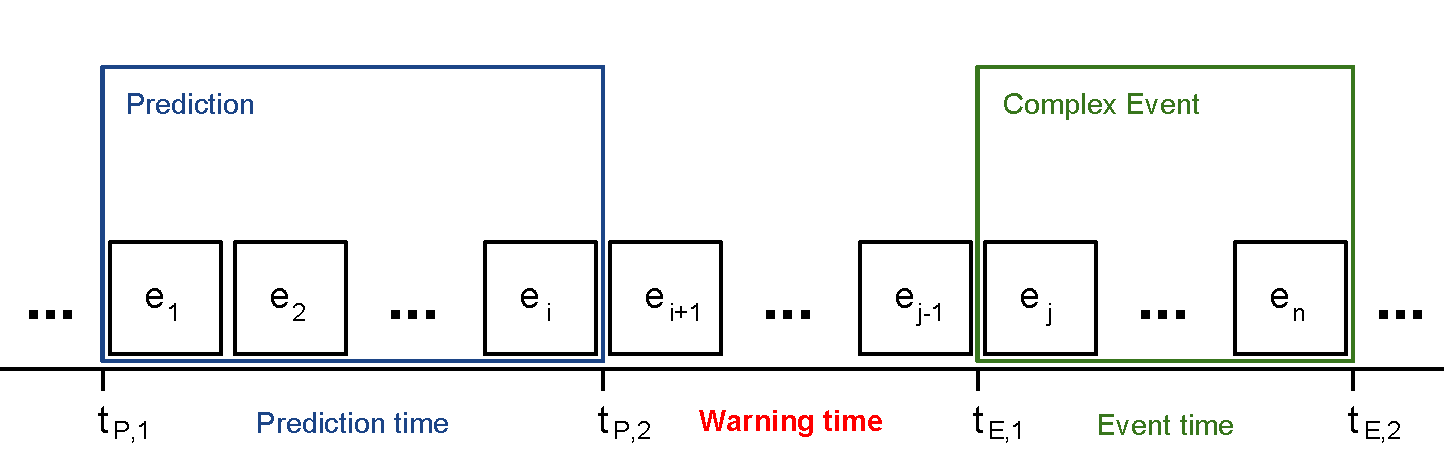
\includegraphics[scale=0.7]{images/prediction_time_span.pdf}
\caption{Timing of complex event prediction.}
\label{fig:prediction_time_span}
\end{figure}

The event history $h = \{e_1, ..., e_i\}$ in the prediction interval is a multivariate time series, that is, it contains a sequence of numerical vectors. \cite{Xing10} Each vector contains the measurement values from different sensor at a certain point in time. I will design the system so that the CEP engine receives every $\Delta t$ seconds a new event that contains the recent measurement values from all the available sensors. The choice of $\Delta t$ depends on the phenomenon investigated, an issue which I will talk about more in Chapter 4.

We can formulate the prediction process as a binary classification task that contains two classes:
\begin{enumerate}
\item{Histories that precede an event}
\item{Histories that do not precede an event}
\end{enumerate} 

We can denote theses classes by $w_1$ and $w_2$.
The task is to learn a classifier $C$, which maps a history $h$ into a class $w$: $C \ : \ h \rightarrow w, \ w \in C$, where 
\begin{eqnarray*}
C &=& \{w_1, w_2\} \label{eq:classification} \\
&=& \{\text{``Event is not going to happen''}, \text{``Event is going to happen''}\}
\end{eqnarray*}

Time series classification methods can be divided into different categories: distance based methods, feature based methods, model based methods and so on. Two of these, distance based and feature based methods are investigated and tested in this thesis. 

From distance based methods I present $L_p$ norms and Dynamic Time Warping (DTW) as distance measures in co-operation with k-Nearest Neighbor (kNN) and Learning Vector Quantization as classification methods. The empirical section of this thesis employs a model that uses DTW and kNN.

From feature based methods I present Fourier and Wavelet analyses for feature extraction and then Support Vector Machines (SVMs) for classifying the feature vectors.



\section{Distance Based Time Series Classification}
Distance based methods are probably the simplest way to classify time series. They rely on a measure function that relates the time series to a single numeric value which indicates the similarity between two different time series. Then, a classification method can be used to separate different classes of time series. \cite{Xing10}

In this chapter I first present $L_p$ norms and Dynamic Time Warping (DTW) as examples of measure functions. Then, k-nearest neighbors (kNN) and learning vector quantization (LVQ) algorithms are formulated for classifying the time series.



\subsection{$L_p$ norms}
One way to classify time series is to calculate a distance measure between a new time series and the existing labeled time series. Then, one can select the group with has the lowest distance with the time series being classified. The easiest approach is some $L_p$ norm which can be calculated for time series $\mathbf{x} = \{x_0, x_1, ..., x_{n-1}\}$ and $\mathbf{y} = \{y_0, y_1, ..., y_{n-1}\}$ with \cite{smith07}

\begin{equation}
D(\mathbf{x}, \mathbf{y}) = \left( \sum_{i=0}^{n-1} \left| x_i - y_i \right|^p \right)^{\frac{1}{p}}.
\end{equation}

Then, one can use various algorithms, such as nearest neighbor classifiers or decision trees, to classify the time series into different groups. Examples of $L_p$ norms are Manhattan norm ($p = 1$), Euclidean norm ($p = 2$) and maximum norm ($p \rightarrow \infty$). $L_p$ norms are very straightforward to calculate but requires normalization of the signals in order to handle similar signals with different amplitudes. \cite{MiningTimeSeriesData} 

\subsection{Dynamic Time Warping}
$L_p$ norms cannot group signals that are, for example, in different phases, no matter how similar they are. One way to overcome this problem is to use dynamic time warping (DTW) algorithm. It measures the similarity between two signals that may vary in time or speed by "warping" the axis of one time series so that the phases of the signals match. \cite{MiningTimeSeriesData} Let us denote a feature space, that is, available values for $x_i$ and $y_j$ by $\digamma$. A classical DTW algorithm begins by creating a matrix 

\begin{equation}
C(i, j) = c(x_i, y_j),
\end{equation}
where $c$ is a local distance measure: $c \ : \ \digamma \times \digamma \rightarrow \mathbb{R}$ that is the difference between the two variables. In other words, the two time series being compared are laid on the two axes of the matrix and the matrix contains the differences between the corresponding values in the time series.

Then, by using dynamic programming, a monotonically increasing minimal path from the bottom left corner of the matrix to the top right corner is searched. The algorithm begins by calculating the cumulative matrix \emph{D} beginning from the bottom left corner of the cost matrix \emph{C}. Then, the minimum path in the cumulative matrix defines the optimal alignment between \emph{x} and \emph{y}. \cite{Muller07} 

The difference between Euclidean distance and DTW distance is illustrated in Figure~\ref{fig:euclidean_vs_dtw}. While Euclidean distance always compares the two time series point by point, DTW distance warps the other time series so that the extrema of the two time series are matched. This gives a more comprehensive similarity measure for two time series.

\begin{figure}[here]
\centering
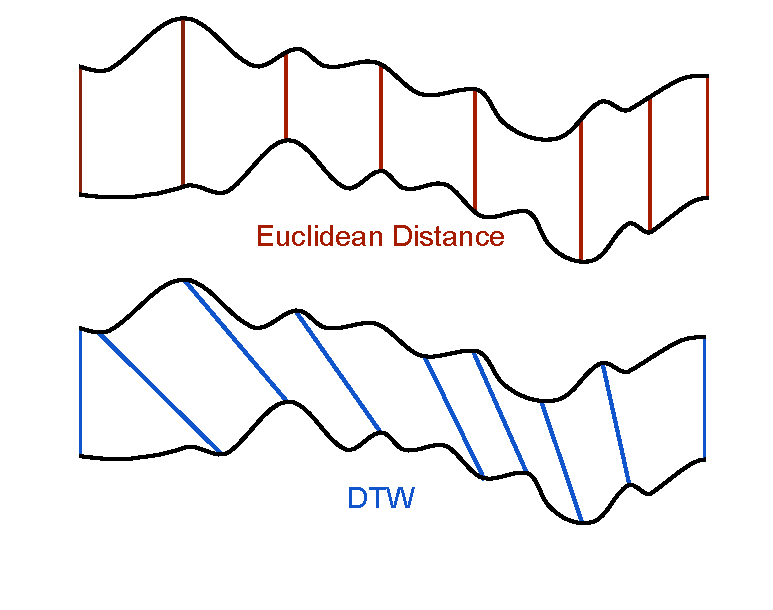
\includegraphics[scale=0.7]{images/euclidean_vs_dtw.pdf}
\caption{Difference between Euclidean Distance and Dynamic Time Warping.}
\label{fig:euclidean_vs_dtw}
\end{figure}



The vertical lines in the figure illustrate the points in the time series that are compared against each other. As can be seen, the algorithm matches the peaks and the valleys with one another. A pseudo code is presented in the following:


\begin{algorithm}[H]
	\KwData{Cost function $c$, Width $N$, Height $M$}
	\KwResult{Optimal Warping Path $p$}	
	Calculate cumulative cost matrix D starting from bottom left corner\;
	Set n = N and m = M\;
	\While{n > 0 and m > 0}{
		Move to neighbor with the smallest D(n, m)\; 
		Store movement to p\;
		Update n and m\;
	}
	reverse $p$\;
	return $p$;
\end{algorithm}


\subsection{k-Nearest Neighbor Algorithm}
Our classifying task consists of two classes as shown in Equation~\ref{eq:classification}. Once we have agreed on which distance measure we are using, we can use k-nearest neighbor (kNN) algorithm to classify new time-series instances. In the experimental chapter of this thesis I use Dynamic Time Warping (DTW) that was introduced in the previous section.

The kNN algorithm is a supervised learning algorithm, which means that we need a labeled teaching set to initialize the algorithm. \cite{PatternRecognition} The time-series in the teaching set have been labeled so that their label is either $w_1$ or $w_2$ depending on which class they belong to. 

Now for every new time-series instance we calculate the distance between the new instance and all the instances in the teaching set. Then, we select the $k$ instances with the least distances to our new instance. These $k$ instances vote for how the new instance is classified: the class with most instances is chosen. Clearly, the parameter $k$ should be odd so that we avoid draws between the two classes. \cite{Hastie08}


\subsection{Learning Vector Quantization}
Learning vector quantization (LVQ) is a supervised neural network that uses winner-take-all prototype-based learning. The LVQ algorithm, first developed by Teuvo Kohonen \cite{Kohonen90}, is similar to the kNN except for the application of moving prototype vectors. The M prototype vectors $\{z_1, ..., z_M\}$ are labeled vectors that represent the classes $C(z_m), m = 1, 2, ..., M$ and can be selected randomly from the set of available training vectors. Then, for each training vector $x_i, i = 1, ..., N$ the nearest prototype vector $z_m$ is updated with the following rule:
\begin{align}
z_m \leftarrow 
\begin{cases}
z_m + \alpha (x_i - z_m), & \text{if $z_m$ and $x_i$ belong to the same class} \\
z_m - \alpha (x_i - z_m), & \text{if $z_m$ and $x_i$ belong to different classes}
\end{cases},
\end{align} 

where $\alpha$ is the learning rate. In other words, the closest prototype vector is moved towards the instance if its from the same class as the prototype vector. In the opposite case, the prototype vector is moved away from the instance. When using the model with testing data, each new instance is classified with the same class as the closest prototype vector.

Usually, the training vectors are iterated through multiple times for a better convergence. On every iteration the value of $\alpha$ can be decreased so the algorithm first takes larger steps and then gradually moves to smaller steps. By doing this it first moves the prototype vectors to correct areas and then refines their positions. \cite{Li08}



\section{Feature Based Time Series Classification}
The aim of feature generation is to transform a sequence of time series data into a single vector that has as few dimensions as possible but still contains the relevant information about the time series for the classifying task. This process is a part of the preprocessing step of machine learning. We do this in order to reduce dimensionality, to increase learning accuracy and to improve result comprehensibility. \cite{Yu03}

There is a clear difference between feature selection and feature extraction. The former means choosing a subset from the available variables and using that as a feature vector, which is not an applicable method in the case of a time series as each variable in our multivariate time series is of a too high dimensionality by itself. The latter means mapping the available data into a lower dimensional space with some algorithm. \cite{Yu03} In sections 3.5.1 and 3.5.2 I present a technique for feature extraction by capturing a subset of the signal spectra with wavelet analysis.

Theoretically we could combine all the time series vectors from the prediction interval into one large feature vector that is then used as an input for the classifier $C$. However, as the prediction interval gets longer, we face the curse of dimensionality. The longer the feature vector is, the sparser the data becomes and the less statistically significant the classifying is. Also, the volume of the data increases rapidly and the processing becomes more and more demanding. \cite{Pascual07} For this reason, I describe a way to reduce the dimensionality of the feature vectors.

\subsection{Wavelet Analysis}
Wavelet analysis is a generalization of Fourier analysis which breaks the signal into series of sines and cosines. This transformation reveals the frequency space properties but loses all the temporal information. \cite{Fong04} A Fourier transform of a function $x(t)$ is 
\begin{equation}
F_{x}(t) = a_0 + \sum_{k=1}^{\infty} a_k cos(kt) + b_k sin(kt),
\end{equation}

where
\begin{align}
a_0 &= \frac{1}{2\pi} \int_{0}^{2\pi} x(t) dt \\
a_k &= \frac{1}{\pi} \int_{0}^{2\pi} x(t) cos(kt) dt \\
b_k &= \frac{1}{\pi} \int_{0}^{2\pi} x(t) sin(kt) dt.
\end{align}

This corresponds to a mapping into the frequency space that is formed by orthogonal basis functions, sine and cosine. By orthogonality we mean that for a set of signals $\psi_n(t)$, $-\infty < n < \infty$, we have
\begin{equation}
\left \langle \psi_n(t), \psi_m(t) \right \rangle = 0, \; m \ne n
\end{equation}

We can generalize the idea of Fourier transform into any orthogonal basis of signals $\psi_n(t)$. The analysis part calculates the coefficients of the original signal $x(t)$ in the new space:
\begin{equation}
c_n = \frac{\left \langle x(t), \psi_n(t) \right \rangle}{\left \langle \psi_n(t), \psi_n(t) \right \rangle}.
\end{equation}

Then, the original signal can be constructed from the coefficients by
\begin{equation}
x(t) = \sum_{n=-\infty}^{\infty} c_n \psi_n(t),
\end{equation}
which is called the synthesis process.

Fourier transform reveals the frequency band of the signal while losing all the temporal information about different frequencies. \cite{Fong04} Because of this Fourier transform is applicable only to stationary signals $f(t)$ whose variance does not vary with time. No information about the changes in variance are captured by Fourier transformation and hence the method becomes useless with non-stationary signals. Anomalies in time series data cause spectral variance and hence the signal is not stationary. \cite{Hautakangas11} 

We can define the short time Fourier transform (STFT) as
\begin{equation}
\operatorname{STFT}(f, s) = \int_{-\infty}^{\infty} x(t) g(t-s) e^{-j 2\pi ft} dt,
\end{equation}
where $f$ is frequency of $x(t)$ and $g(t)$ is a sliding window function, for example, a box function
\begin{equation}
\operatorname{box}(t) = 
\begin{cases}
1 & \text{for} \; |t| \le 1/2 \\
0 & \text{elsewhere}
\end{cases}.
\end{equation}

This restricts the Fourier transform into one window at the time and thus achieves time-localization which the ordinary Fourier transform lacks of. For computational purposes we must discretize this by denoting $f_n = n/T$ and $s_m = mT$. In this case our orthogonal basis functions are
\begin{equation}
v_{n,m} (t) = e^{j 2\pi nt / T} g(t - mT).
\end{equation}

Now the analysis part is
\begin{align}
c_{n,m} &= \frac{\left \langle x(t), v_{n,m}(t) \right \rangle}{\left \langle v_{n,m}(t), v_{n,m}(t) \right \rangle} \\
&= \frac{1}{T} \int_{mT}^{(m+1)T} x(t) e^{-j 2\pi nt / T} dt
\end{align}
and the synthesis is 
\begin{equation}
x(t) = \sum_{n=-\infty}^{\infty} \sum_{m=-\infty}^{\infty} c_{n,m} e^{j 2\pi nt / T} g(t - mT).
\end{equation}

Unlike Fourier transform, wavelet transformation gives the signal localization in both time and frequency spaces. It does this by using a concept called multi-resolution analysis (MRA) which means that different frequencies are analyzed with different resolutions. While Fourier transformation uses equally-sized windows for all frequencies, Wavelet transformation uses longer time windows for low frequencies and shorter time windows for high frequencies. This approach allows good localization of high frequency components while preserving information about low frequency contents of the signal. \cite{Fong04}

Continuous wavelet transform (CWT) for signal $x(t)$ is defined as
\begin{equation}
C_{x}(a,b) = \frac{1}{\sqrt{|a|}} \int_{-\infty}^{\infty} x(t) w \left ( \frac{t - b}{a} \right ) dt,
\end{equation}
where $a$ and $b$ are scaling and positioning parameters and $w(t)$ is a so-called mother wavelet function. \cite{Fong04} 

For computational purposes we must find a discrete wavelet transform (DWT). By choosing the scales to be powers of 2 and the positions to be multiples of the scales, we get an orthogonal basis of functions for CWT:
\begin{equation}
w_{j,k}(t) = 2^{j/2} w(2^j t - k).
\end{equation}

These $w_{j,k}(t)$ are called the baby wavelets. \cite{Phillips03} As can be easily seen, baby wavelets become narrower and higher as the $j$ increases. The reverse is also true, baby wavelets become wider and flatter as the $j$ decreases. We can now define space $W_j$ to contain all the signals $x_j(t)$ that can be synthesized from baby wavelets $w_{j,k}(t)$ with the $j$ fixed:
\begin{equation}
x_j(t) = \sum_{k=-\infty}^{\infty} c_{j,k} w_{j,k}(t).
\end{equation}

Similarly, let $V_j$ to be the space of signals $x(t)$ that can be synthesized from baby wavelets $w_{i,k}(t)$ where $i < j$ and $-\infty < k < \infty$. Then, from the definition of $W_j$ and $V_j$ we have $V_{j+1} = W_j + V_j$. This is illustrated in figure~\ref{fig:wavelet_spaces}.


\begin{figure}[here]
\centering
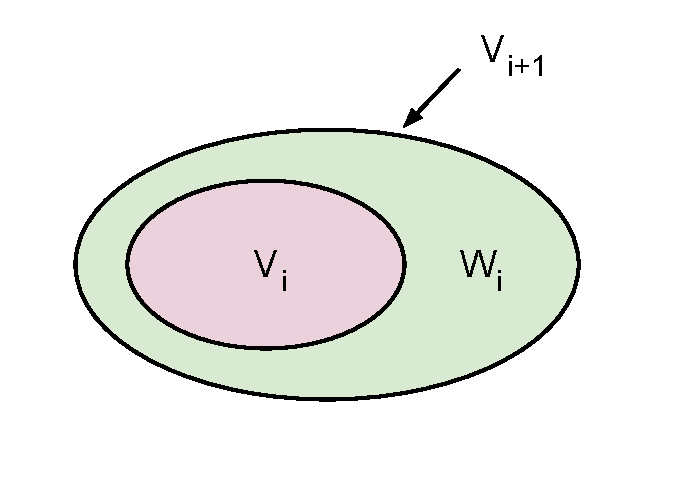
\includegraphics[scale=0.7]{images/wavelet_spaces.pdf}
\caption{Wavelet subspaces.}
\label{fig:wavelet_spaces}
\end{figure}

Thus, the spaces $V_j$ are nested inside each other, that is $\{0\} \subset \ldots \subset V_{-1} \subset V_{0} \subset V_{1} \subset \ldots L^2$, where $L^2$ contains all possible signals. The spaces $W_j$ are the differences between adjacent spaces $V_j$ and $V_{j+1}$. Now we can divide the space $V_0$ as
\begin{align*}
V_0 &= V_{-1} + W_{-1} \\
&= V_{-2} + W_{-2} + W_{-1} \\
&= V_{-3} + W_{-3} + W_{-2} + W_{-1} \\
&= \cdots
\end{align*}
and the signal as
\begin{align}
x(t) &= A_1(t) + D_1(t) \label{eq:decomposition} \\
&= A_2(t) + D_2(t) + D_1(t) \\
&= A_3(t) + D_3(t) + D_2(t) + D_1(t) \\
&= \cdots,
\end{align}
where $D_i(t) \in W_{-i}$ is the detail at level $i$ and $A_i(t) \in V_{-i}$ is the approximation at level $i$. This approach is called multi-resolution analysis (MRA) because on each step we divide the frequency band into two pieces and then continue the process on the lower half. At each stage the $A_i(t)$ corresponds to low-pass filtered signal and the $D_i(t)$ to high-pass filtered signal. This way we get more detailed information about the high frequencies. \cite{Phillips03} 

To facilitate the computations we can define a scaling function $\phi(t)$ (sometimes called the father wavelet) which produces the subspaces $V_j$:
\begin{equation}
\phi_{j,k}(t) = \sqrt{2^j} \phi(2^j t - k).
\end{equation}

Because $V_0 \subset V_1$ and $W_0 \subset V_1$, it is possible to construct the mother wavelet and the scaling function in $V_1$ from the scaling function in $V_0$ as follows
\begin{align}
\phi(t) &= \sum_n h_0(n) \sqrt{2} \phi(2t - n) \\
w(t) &= \sum_n h_1(n) \sqrt{2} \phi(2t - n),
\end{align}
where $h_0(n)$ and $h_1(n)$ are discrete time filter coefficients. These depend on the choice of wavelet type and they will be defined later. Now we are able to define the signal $x(t) \in V_j$ using the mother wavelet and the scaling function in spaces $V_{j-1}$ and $W_{j-1}$
\begin{align}
x(t) &= \sum_k cA_0(k) \phi_{j,k}(t) \\
&= \sum_k cA_1(k) \phi_{j-1,k}(t) + \sum_k cD_1(k) w_{j-1,k}(t) \\
&= A_1(t) + D_1(t),
\end{align}
where $cA_0(k)$, $cA_1(k)$ and $cD_1(k)$ are the approximate and detail coefficients respectively. Then, $\phi_{j-1,k}$ can be further filtered to get the next level signals as shown in equation~\ref{eq:decomposition}. The coefficient values can be derived as follows
\begin{align}
cA_1(k) &= \left \langle x(t), \phi_{j-1,k}(t) \right \rangle \\
		&= \left \langle \sum_n cA_0(n) \phi_{j,n}(t), \phi_{j-1,k}(t) \right \rangle \\
		&= \sum_n cA_0(n) \left \langle \phi_{j,n}(t), \phi_{j-1,k}(t) \right \rangle,
\end{align}
which, by calculating the inner product simplifies to
\begin{align}
cA_1(k) = \sum_n h_0(n-2k) cA_0(n)
\end{align}

Similarly, for $cD_1(k)$ we get
\begin{align}
cD_1(k) = \sum_n h_1(n-2k) cA_0(n)
\end{align}

These two operations correspond to filters
\begin{align}
&cA_0(n) \longrightarrow \boxed{h_0(-n)} \longrightarrow \boxed{\downarrow 2} \longrightarrow cA_1(k) \label{eq:downsampling1} \\
&cA_0(n) \longrightarrow \boxed{h_1(-n)} \longrightarrow \boxed{\downarrow 2} \longrightarrow cD_1(k), \label{eq:downsampling2}
\end{align}
where the downsampling filter, $\boxed{\downarrow 2}$, means omitting every other value from the signal. As shown in equation~\ref{eq:decomposition}, we can further use the downsampling filters to decompose the signal into more detail. This process is shown in Figure~\ref{fig:wavelet_filters}.

\begin{figure}[here]
\centering
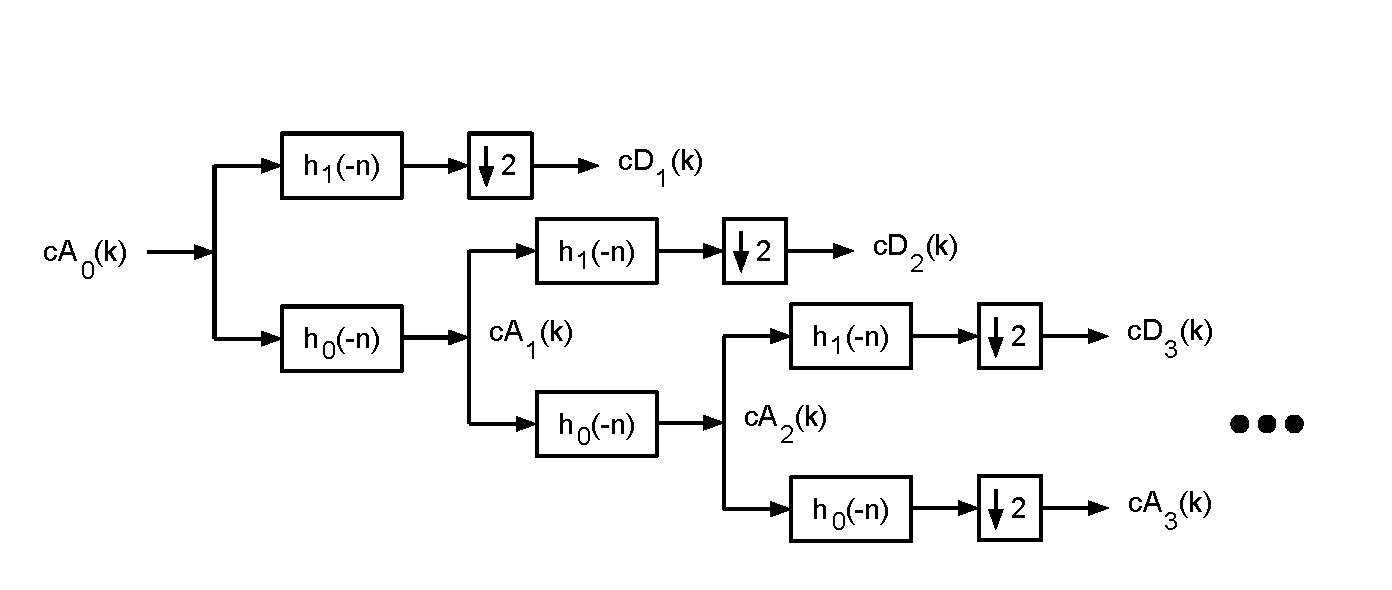
\includegraphics[scale=0.7]{images/wavelet_filters.pdf}
\caption{Wavelet coefficient decomposition using filters.}
\label{fig:wavelet_filters}
\end{figure}

Now on level $N$ our coefficients are
\begin{align}
C = [cA_N, cD_N, cD_{N-1}, ..., cD_2, cD_1]
\end{align}

The signal is now compressed by setting some of the detail coefficients to zero. Of course, the energy of the signal is not completely preserved and the number of zero coefficients depends on the application.

Next, we need to perform the synthesis part by opposite, upsampling filters. This process is shown in Figure~\ref{fig:wavelet_filters2}.

\begin{figure}[here]
\centering
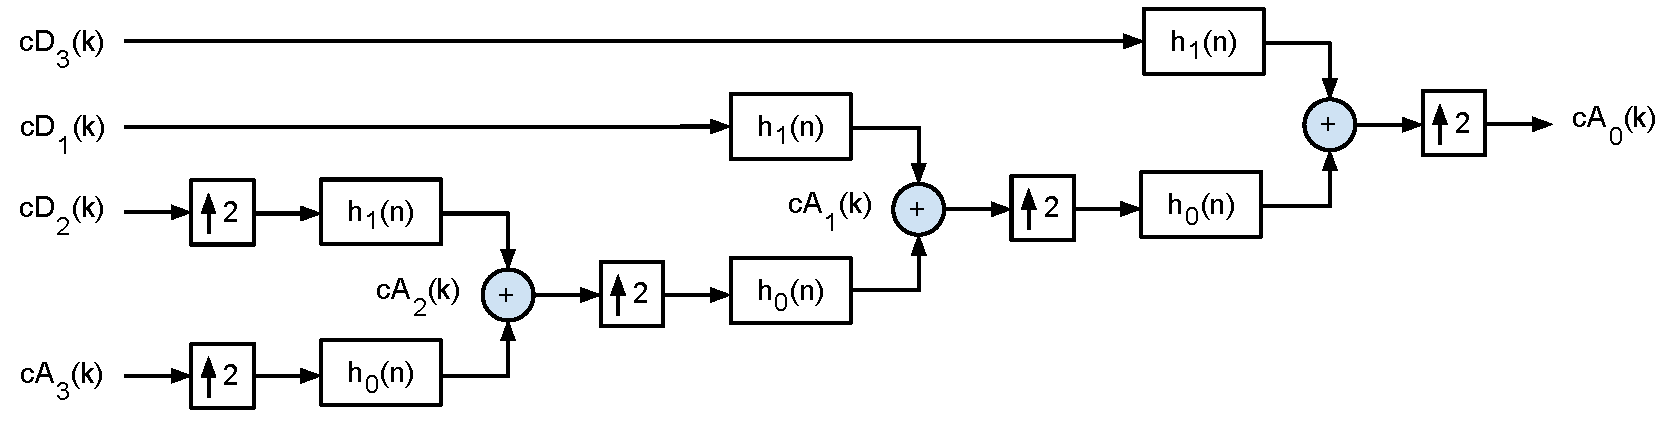
\includegraphics[scale=0.55]{images/wavelet_filters2.pdf}
\caption{Wavelet coefficient decomposition using filters.}
\label{fig:wavelet_filters2}
\end{figure}

If no coefficients are set to zero in the analysis phase, the signal that is constructed in the synthesis phase is exactly the same as the original signal. By setting some of the detail coefficients to zero before the synthesis, some energy of the signal is lost but at the same time the signal is compressed to a smaller size.


\subsection{Haar Wavelet Decomposition for Time Series}
Haar wavelet \cite{struzik99} is the simplest possible wavelet and it has the following mother wavelet 
\begin{align}
\psi(t) = 
\begin{cases}
1, & 0 \le t < 1/2 \\
-1, & 1/2 \le t < 1 \\
0, & otherwise
\end{cases}.
\end{align}

and the following scaling function
\begin{align}
\phi(t) = 
\begin{cases}
1, & 0 \le t < 1 \\
0, & otherwise
\end{cases}.
\end{align}

For Haar wavelets the discrete time filter coefficients $h_0(n)$ and $h_1(n)$ are defined as
\begin{align}
h_0 &= \left [ \frac{1}{\sqrt{2}}, \frac{1}{\sqrt{2}} \right ] \\
h_1 &= \left [ \frac{1}{\sqrt{2}}, -\frac{1}{\sqrt{2}} \right ].
\end{align}

Now let's assume we have a time-series $\mathbf{x} = (x_1, x_2, ..., x_N)$ of length $N = 2^n$. The 1-level Haar-Transform is
\begin{align}
\mathbf{x} \longleftrightarrow (A_1 | D_1),
\end{align}
where 
\begin{align}
A_1 &= \left ( \frac{x_1 + x_2}{\sqrt{2}}, \frac{x_3 + x_4}{\sqrt{2}}, ..., \frac{x_{N-1} + x_N}{\sqrt{2}} \right ) \\
D_1 &= \left ( \frac{x_1 - x_2}{\sqrt{2}}, \frac{x_3 - x_4}{\sqrt{2}}, ..., \frac{x_{N-1} - x_N}{\sqrt{2}} \right ).
\end{align}

The former operation corresponds to a running average (trend) and the latter to a running difference (fluctuation). Then, $A_1$ can be further decomposed into $A_2$ and $D_2$ by performing the same operation again:
\begin{align}
\mathbf{x} \longleftrightarrow (A_2 | D_2 | D_1).
\end{align}

This process is then repeated until a desired level is reached. The Wavelet can be compressed by setting some of the detail coefficients to zero. The resulting vector can now be used as a feature. In the next chapters I describe how these features can be classified with first linear classifiers and then with support vector machines (SVMs) that generalize into nonlinear cases.




\subsection{Linear Classifiers}
In this section I discuss the special case of linearly separable classes. If the input space is linearly separable, we can use a linear hyperplane to separate the two classes. \cite{tappen10} As explained in Chapter 3.3, we have two classes, $w_1$ and $w_2$, for which the $l$-dimensional hyperplane is

\begin{equation}
g(\mathbf{x}) = \mathbf{w}^T \mathbf{x} + w_0 = 0,
\end{equation}
where $\mathbf{x}$ is a feature vector, $\mathbf{w}$ is the weight vector, and $w_0$ is the threshold. The threshold value is needed to cover the case of the hyperplane not crossing the origin. We can extend the vectors into $(l+1)$-dimensional space by defining
\begin{eqnarray}
\mathbf{x'} = \left [ \mathbf{x}^T, 1 \right ]^T \\
\mathbf{w'} = \left [ \mathbf{w}^T, w_0 \right ]^T.
\end{eqnarray}

From now on the variables $\mathbf{x}$ and $\mathbf{w}$ refer to $\mathbf{x'}$ and $\mathbf{w'}$. Now the feature vectors $x$ have the properties
\begin{eqnarray}
\mathbf{w}^T \mathbf{x} > 0 &\;\;& \forall \mathbf{x} \in w_1 \\
\mathbf{w}^T \mathbf{x} < 0 &\;\;& \forall \mathbf{x} \in w_2.
\end{eqnarray}

The problem is now the choice of the weight vector $w$. One way to tackle the problem is the perception algorithm which defines a perception cost as
\begin{equation}
J(\mathbf{w}) = \sum_{\mathbf{x} \in Y} (\delta_x \mathbf{w}^T \mathbf{x}),
\end{equation}
where $Y$ is the set of training vectors that are misclassified with the weigh vector $w$ and $\delta_x = -1$ if $\mathbf{x} \in w_1$ and $\delta_x = +1$ if $\mathbf{x} \in w_2$. Since the cost $J(\mathbf{w})$ is always positive, continuous and piecewise linear, it can be minimized with a gradient descent method \cite{tappen10}:
\begin{eqnarray}
\mathbf{w(t+1)} &=& \mathbf{w(t)} - \rho_t \frac{\partial J(\mathbf{w})}{\partial \mathbf{w}} \\
&=& \mathbf{w(t)} - \rho_t \sum_{\mathbf{x} \in Y} \delta_x \mathbf{x}.
\end{eqnarray}

The iteration is performed until all the training instances have been classified correctly. A variation of perception algorithm loops through the training instances one by one and updates the weight vector on each instance.

Even though the classes are not linearly separable, we can find an optimal linear classifier that minimizes the classification error in some sense. One way to find the optimal $w$ is to use mean square error estimation which tries to minimize the cost function
\begin{equation}
J(\mathbf{w}) = E[|y - \mathbf{x}^T \mathbf{w}|^2],
\end{equation}  

where $y$ is the desired output; in this case $y = 1$ for $w_1$ and $y = -1$ for $w_2$. \cite{gutierrez11} A required condition for the minimum is
\begin{equation}
\frac{\partial J(\mathbf{w}}{\partial \mathbf{w}} = 2 E[\mathbf{x}(y - \mathbf{x}^T \mathbf{w})] = 0.
\end{equation}

The optimal weigh vector is then
\begin{equation}
\mathbf{w} = R_x^{-1} E[\mathbf{x}y],
\end{equation}
where $R_x$ is the correlation matrix of $\mathbf{x}$ and $E[\mathbf{x}y]$ is the cross-correlation vector that have to be estimated from the learning set.

Another way is to use least squares methods that use the cost function
\begin{equation}
J(\mathbf{w}) = \sum_{i=1}^N (y_i - \mathbf{x}_i^T \mathbf{w})^2 = \sum_{i=1}^N e_i^2
\end{equation} 

Then, by differentiating with respect to $\mathbf{w}$ we get
\begin{eqnarray}
&& \sum_{i=1}^N \mathbf{x}_i (y_i - \mathbf{x}_i^T \mathbf{w}) = 0 \\
&\Leftrightarrow& (\sum_{i=1}^N \mathbf{x}_i \mathbf{x}_i^T) \mathbf{w} = \sum_{i=1}^N (\mathbf{x}_i y_i) \\
&\Leftrightarrow& (\mathbf{X}^T \mathbf{X}) \mathbf{w} = \mathbf{X}^T \mathbf{y} \\
&\Leftrightarrow& \mathbf{w} = (\mathbf{X}^T \mathbf{X})^{-1} \mathbf{X}^T \mathbf{y},
\end{eqnarray}
where $\mathbf{X} = [\mathbf{x}_1, ..., \mathbf{x}_N]^T$, $\mathbf{y} = [y_1, ..., y_N]^T$, and $\mathbf{X}^T \mathbf{X}$ is sample correlation matrix which can be estimated from the available data. \cite{gutierrez11}




\subsection{Support Vector Machines for Linearly Separable Classes}
The following three chapters follow the support vector machine chapters 3.7 and 4.18 discussed in the book \emph{Pattern recognition} by Theodoridis and Koutroumbas \cite{PatternRecognition}.

I first discuss the Support Vector Machines in case of two linearly separable classes. Similarly to the previous section with linear classifiers, we design a hyperplane
\begin{equation}
g(\mathbf{x}) = \mathbf{w}^T \mathbf{x} + w_0 = 0
\end{equation}

\begin{figure}[here]
\centering
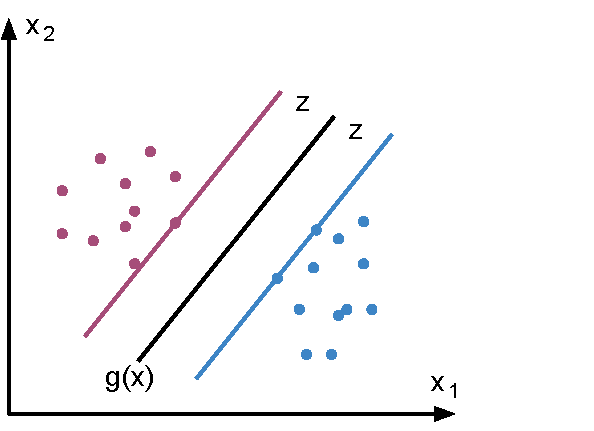
\includegraphics[scale=0.7]{images/svm_linear.pdf}
\caption{Maximum separating hyperplane between two linearly separable classes.}
\label{fig:svm_linear}
\end{figure}

When the hyperplane leaves maximal margins between the class instances and itself, the performance of classifier is optimal. This situation is depicted in Figure~\ref{fig:svm_linear}. Thus, we should maximize the margin $z$ which can be represented as $z = |g(\mathbf{x})| / ||\mathbf{w}||$. If we scale $\mathbf{w}$ and $w_0$ so that $g(\mathbf{x}) = 1$ for the class $w_1$ and $g(\mathbf{x}) = -1$ for the class $w_2$ on the points that are closest to the hyperplane, we have a margin of $2 / ||\mathbf{w}||$ and requirements
\begin{align}
\mathbf{w}^T \mathbf{x} + w_0 \ge 1, &\; \forall \mathbf{x} \in w_1 \\
\mathbf{w}^T \mathbf{x} + w_0 \le -1, &\; \forall \mathbf{x} \in w_2
\end{align}

We can form the problem as the following optimization problem
\begin{align}
\text{minimize} &\; J(\mathbf{w}, w_0) = \frac{1}{2} ||\mathbf{w}||^2 \\
\text{subject to} &\; y_i (\mathbf{w}^T \mathbf{x}_i + w_0) \ge 1, \; i = 1,2,...,N \label{eq:svm_linear_variables} 
\end{align}
where $y_1 = 1$ and $y_2 = -1$. The Karush-Kuhn-Tucker (KKT) conditions for this nonlinear quadratic optimization problem are
\begin{eqnarray} 
L_{\mathbf{w}}(\mathbf{w}, w_0, \mathbf{\lambda}) &=& \mathbf{0} \label{eq:KKT} \\
L_{w_0}(\mathbf{w}, w_0, \mathbf{\lambda}) &=& 0 \\
\lambda_i &\ge& 0, \; i = 1, 2, ..., N \\
\lambda_i [y_i (\mathbf{w}^T \mathbf{x}_i + w_0) - 1] &=& 0,
i = 1, 2, ..., N,
\end{eqnarray}
where $L(\mathbf{w}, w_0, \mathbf{\lambda})$ is the Lagrangian function
\begin{equation}
L(\mathbf{w}, w_0, \mathbf{\lambda}) = \frac{1}{2} \mathbf{w}^T \mathbf{w} - \sum_{i=1}^N \lambda_i [y_i (\mathbf{w}^T \mathbf{x}_i + w_0) - 1]
\end{equation}

Solving the first order differential equations in the KKT conditions yields a dual problem
\begin{eqnarray}
\text{maximize} &\;& L(\mathbf{w}, w_0, \lambda) \\
\text{subject to} &\;& \mathbf{w} = \sum_{i=1}^N \lambda_i y_i \mathbf{x}_i \\
&& \sum_{i=1}^N \lambda_i y_i = 0 \\
&& \mathbf{\lambda} \ge \mathbf{0}
\end{eqnarray}

By substituting the first two conditions into the Lagrangian $L$ we further get
\begin{eqnarray}
&\underset{\mathbf{\lambda}}{\operatorname{max}}& \left ( \sum_{i=1}^N \lambda_i - \frac{1}{2} \sum_{i, j} \lambda_i \lambda_j y_i y_j \mathbf{x}_i^T \mathbf{x}_j \right ) \label{eq:SVM_KKT_1} \\ 
&\text{subject to}& \sum_{i=1}^N \lambda_i y_i = 0 \label{eq:SVM_KKT_2} \\ 
&&\mathbf{\lambda} \ge 0 \label{eq:SVM_KKT_3}
\end{eqnarray}

As we can easily see, the function to be maximized does not depend on the dimensionality of the input space because it contains the input vectors in the form of a inner product. This allows us to easily generalize the method into non-separable classes by mapping them into a higher-dimensional space in the next sections.

The Support Vectors are the points $\mathbf{x}_i$ for which the Lagrangian multiplier $\lambda_i$ is not zero and which lie on one of the hyperplanes $\mathbf{w}^T \mathbf{x} + w_0 = \pm 1$. The optimal hyperplane of SVM is unique because the cost function in equation~\ref{eq:KKT} is strictly convex.


\subsection{Support Vector Machines for Linearly Non-separable Classes}
Now we turn to the case of classes that cannot be separated with a linear hyperplane. In this case we introduce slack variables $\xi_i \ge 0$ that allow some points to fall on the wrong side of the hyperplane. Now the equation~\ref{eq:svm_linear_variables} is replaced with
\begin{equation}
y_i [\mathbf{w}^T \mathbf{x} + w_0] \ge 1 - \xi_i,
\end{equation}  
where the value of $\xi_i$ defines the type of the point as follows:
\begin{enumerate}
\item $\xi_i = 0$ $\Rightarrow$ Point is classified correctly.
\item $0 < \xi_i \le 1$ $\Rightarrow$ Point is classified correctly but it is on the wrong side of the margin.
\item $\xi_i > 1$ $\Rightarrow$ Point is misclassified.
\end{enumerate}

These three types are illustrated in figure~\ref{fig:svm_non_separable}. An yellow ring marks a point that is classified correctly but that is on the wrong side of the margin (type 2). A red square marks a point that is misclassified (type 3).  

\begin{figure}[here]
\centering
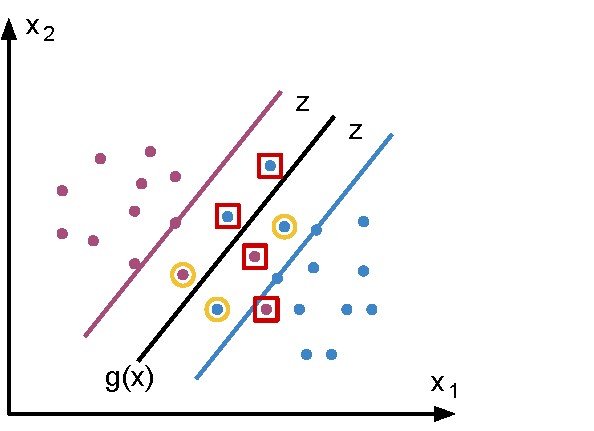
\includegraphics[scale=0.7]{images/svm_non_separable.pdf}
\caption{A separating hyperplane between two classes that are non-separable. A yellow ring marks a point that is classified correctly but that is on the wrong side of the margin. A red square marks a point that is misclassified.}
\label{fig:svm_non_separable}
\end{figure}

In this case our optimization problem can be stated as
\begin{align}
\text{minimize} &\; J(\mathbf{w}, w_0, \mathbf{\xi}) = \frac{1}{2} ||\mathbf{w}||^2 + C \sum_{i=1}^N I(\xi_i) \label{eq:SVM_C_parameter} \\
\text{subject to} &\; y_i [\mathbf{w}^T \mathbf{x}_i + w_0] \ge 1 - \xi_i, i = 1, 2, ..., N \\
& \xi_i \ge 0, i = 1, 2, ..., N,
\end{align}
where $I(\xi_i) = 1$ if $\xi_i > 0$ and $I(\xi_i) = 0$ if $\xi_i = 0$ and the parameter $C$ defines a trade-off between maximizing the margin and minimizing the number of misclassified points. Similarly to the previous section, we can build a dual problem that leads to the problem
\begin{align}
\underset{\mathbf{\lambda}}{\operatorname{max}} &\; \left ( \sum_{i=1}^N \lambda_i - \frac{1}{2} \sum_{i,j} \lambda_i \lambda_j y_i y_j \mathbf{x}_i^T \mathbf{x}_j \right ) \\
\text{subject to} &\; 0 \le \lambda_i \le C, i = 1, 2, ..., N \\
&\; \sum_{i=1}^N \lambda_i y_i = 0.
\end{align}

Again, the dimensionality of the input space disappears from the problem and the input vectors appear only as inner products. There is a shortcut for calculating these inner products with a kernel trick \cite{Jordan04}, which is described in the next section.

\subsection{Generalization of SVMs into Nonlinear Cases}
\begin{figure}[here]
\centering
\includegraphics[scale=0.7]{images/svm_mapping.pdf}
\caption{The main idea of Support Vector Machines. Classes are not linearly separable in the input space. They are mapped into a higher-dimensional space where a linear classifier can be formed. This classifier corresponds to a non-linear classifier in the original input space.}
\label{fig:svm_mapping}
\end{figure}


If the classes are not separable in the $l$-dimensional input space, we can find a mapping $\mathbf{x} \in \mathbb{R}^l \; \rightarrow \; \mathbf{y} \in \mathbb{R}^k$, where $k > l$. The choice of $k$ is done so that the original classes are linearly separable in the new, higher-dimensional space. This situation is depicted in Figure~\ref{fig:svm_mapping}. As mentioned in the previous chapters, our optimization problems contain input vector $x$ only as an inner product that is not altered by the mapping.

In order to present the Mercer's Theorem \cite{Jordan04} that relates the inner product to a kernel function, we need to explain some space related concepts. A Cauchy sequence is defined as a sequence $a_1, a_2, ...$ for which
\begin{equation}
\forall \epsilon \in \mathbb{R} \; \exists \; N > 0  \; s.t.  \; |a_m - a_n| < \epsilon, \; m, n > N
\end{equation}
In other words, the elements of the sequence become arbitrarily close as the sequence progresses. A complete space is a space where every Cauchy sequence converges to a point that is also contained within the space. A Hilbert space, in turn, is a generalization of Euclidean space into any finite or infinite number of dimensions. It is a complete vector space that has inner product defined for measuring lengths and angles. \cite{duchateau02}

Mercer's Theorem states that for each mapping $\mathbf{x} \rightarrow \mathbf{\phi}(\mathbf{x}) \in H$, where $H$ is a Hilbert Space, we have a kernel function $K(\mathbf{x}, \mathbf{y})$ that is equivalent for the inner product:
\begin{equation}
\left \langle \mathbf{\phi}(\mathbf{x}), \mathbf{\phi}(\mathbf{y}) \right \rangle = K(\mathbf{x}, \mathbf{y}).
\end{equation}

The kernel function must have the following properties
\begin{align}
\int_S \int_S K(\mathbf{x}, \mathbf{y})g(\mathbf{x})g(\mathbf{y})d\mathbf{x}d\mathbf{y} &\ge 0 \\ 
\int_S g(\mathbf{x})^2 d\mathbf{x} &< +\infty, \; \forall g(\mathbf{x}), \mathbf{x} \in S, 
\end{align}
where $S \subset \mathbb{R}^l$. The opposite is also true: for any Kernel function satisfying the conditions above there is a Hilbert space where the Kernel function is equivalent for the inner product. The problem is now how to find the mapping $\phi$ when we have selected the Kernel function.

Now we can replace the inner product in Equation~\ref{eq:SVM_KKT_1} with the Kernel function to get the optimization problem
\begin{align}
\underset{\mathbf{\lambda}}{\operatorname{max}} &\left ( \sum_i \lambda_i - \frac{1}{2} \sum_{i,j} \lambda_i \lambda_j y_i y_j K(\mathbf{x}_i, \mathbf{x}_j) \right ) \label{eq:SVM_final_problem} \\
\text{subject to} &\; 0 \le \lambda_i \le C, \; i = 1, 2, ..., N \\
&\; \sum_i \lambda_i y_i = 0.
\end{align}

The resulting non-linear classifier is then
\begin{equation}
g(\mathbf{x}) = \sum_{i=1}^{N_s} \lambda_i y_i K(\mathbf{x}_i, \mathbf{x}) + w_0 \begin{cases}
> 0, \; \Rightarrow \mathbf{x} \in w_1 \\
< 0, \; \Rightarrow \mathbf{x} \in w_2,
\end{cases} \label{eq:SVM_classifier}, 
\end{equation}
which is shown in Figure~\ref{fig:svm_network}. Input vectors enter the network from the left. Then, inner products are calculated in middle nodes, the number of which is N, the number of support vectors. An output node sums the components up and outputs a single real number that determines the result of the classification according to equation~\ref{eq:SVM_classifier}.


\begin{figure}[here]
\centering
\includegraphics[scale=0.7]{images/svm_network.pdf}
\caption{SVM classifier as a network. Input vectors enter the network from the left. Kernel functions calculate inner products in the middle nodes. Output node combines sums the components up and outputs a single real number.}
\label{fig:svm_network}
\end{figure}



\subsection{Using SVM for Time Series Analysis}
Before we can use our SVM classifier, we have to choose an appropriate kernel function $K(\mathbf{x}, \mathbf{y})$ for classifying wavelet based feature vectors. In literature one of the most used kernels is the Gaussian kernel \cite{Zhang04}, which is of the form
\begin{equation}
K(\mathbf{x}, \mathbf{y}) = \exp{\frac{||\mathbf{x} - \mathbf{y}||^2}{2\gamma^2}}, \label{eq:RBF_kernel},
\end{equation}
where $\beta > 0$ is a parameter chosen by the user. Gaussian kernel belongs to a family of functions called radial basis functions (RBF) whose value depends only on the distance between two points \cite{Scholkopf97}
\begin{equation}
f(\mathbf{x}, \mathbf{y}) = f(||\mathbf{x} - \mathbf{y}||)
\end{equation}

If we assume that the time series is generated by an AR(1)-process 
\begin{align}
x_T = g(x_{T-1}, ..., x_{T-k}) + \mu,
\end{align}
it can be shown that an ellipsoid with mean equal to the mean of the time series and variance equal to $\mu$ contains most of the data. The variable $\mu$ is a Gaussian noise component. Consequently, similar time windows are close to each other in the sense of Euclidean Distance. This makes RBF Kernels promising for time series analysis. \cite{Ruping01}

Another possibility is Polynomial Kernel that is of the form
\begin{equation}
K(\mathbf{x}, \mathbf{y}) = (\mathbf{x}^T \mathbf{y} + c)^d,
\end{equation}
which gives the Linear Kernel as a special case when $d = 1$. \cite{Scholkopf97}

Subsequence Kernels look for informative subsequences that are similar in dependent time windows. In this case the Kernel function becomes
\begin{equation}
K(\mathbf{x}, \mathbf{y}) = \sum_{s_x, s_y} K (s_x, s_y),
\end{equation}
where $s_x$ and $s_y$ are subsequences of x and y. There are $\binom{n}{k}^2$ possible combinations for time series of length $n$ and subsequence of length $k$, so one must use another algorithm for selecting the optimal subsequences. \cite{Ruping01}

In thesis I use Gaussian RBF Kernels because of their widespread use and good applicability to time series analysis. Ruping \cite{Ruping01} compared Linear, RBF, Fourier, Subsequence and Hidden Markov Model Kernels and came into conclusion that RBF Kernels perform very well on time series learning tasks. However, he recommends to investigate other possibilities in very specialized applications.

A well defined kernel function increases the performance of the SVM greatly and thus Kernel selection is an important part of SVM development \cite{Fong04}. In the case of RBF Kernels we must choose the value of $\gamma$ in \ref{eq:RBF_kernel}. From now on I try to find an optimal value for $\sigma$, which then defines the $\gamma$ from $\gamma = 1 / 2\sigma^2$. The value of $\sigma$ should be chosen so that it minimizes the error
\begin{equation}
E(\sigma) = \sum_{i=1}^N \left | g(\mathbf{x}_i, \sigma) - y_i \right |^2 \label{eq:SVM_error}
\end{equation}

A related theorem states that for a Support Vector Classifier (SVC) there exists a range $[\sigma_A, \sigma_B]$ for which
\begin{align}
&\forall \; \epsilon > 0 \;\; \text{and} \;\; \forall \; \sigma_1, \sigma_2 \in [\sigma_A, \sigma_B] \\
& \left | \sum_{i=1}^N \left | g(\mathbf{x}_i, \sigma_1) - y_i \right | - \sum_{i=1}^N \left | g(\mathbf{x}_i, \sigma_2) - y_i \right | \right | < \epsilon,
\end{align}
where $g(\mathbf{x}_i, \sigma_i)$ is the discriminant function from Equation~\ref{eq:SVM_classifier} and $y_i$ is the desired output ($\pm 1$) \cite{Wenjian08}. In other words, there is a range for $\sigma$ where the Gaussian Kernel's generalization performance is stable. 

To summarize our parameter estimation problem, we have two unknown parameters, Gaussian Kernel parameter $\gamma$ and SVM weighting parameter $C$ from \ref{eq:SVM_C_parameter}. Now there are two ways to find the optimal values for the parameters: gradient search and grid search. Staelin \cite{Staelin03} compared these two methods and came into the conclusion that they both achieve similar results in terms of accuracy. The only difference is clearly the computational cost that is much greater for the grid search. 

To keep things simple, only the grid search is employed in this thesis. The grid is formed as follows
\begin{align}
\ln{\gamma} &\in \left \{ \ln{\gamma_0} - a_0, \ln{\gamma_0} - a_0 + 1, ..., \ln{\gamma_0}, ..., \ln{\gamma_0} + a_0 \right \} \label{eq:svm_gamma} \\
\ln{C} &\in \left \{ 0, 1, ..., C_0 \right \}, \label{eq:svm_c}
\end{align}
where the parameters $\gamma_0$ and $C_0$ have to be chosen. Jaakkola's heuristics \cite{Jaakkola99} give us a initial guess for $\gamma_0$. Let $S$ be our training set. Then, from the set
\begin{equation}
G = \left \{ \lVert \mathbf{x}_i - \mathbf{x}_j \rVert \; | \; (\mathbf{x}_i, y_i), (\mathbf{x}_j, y_j) \in S, y_i \ne y_j \right \}
\end{equation}
we can compute
\begin{equation}
\sigma_0 = \sigma_{Jaakkola} = \operatorname{median}(G)
\end{equation}
and finally $\gamma_0 = 1 / \sigma_0^2$. The parameters $a_0$ and $C_0$ are chosen in the implementation chapter.

%K-fold Cross-Validation (K-CV) can be used to choose the optimal values for $\gamma$ and $C$ from the grid. First, we divide our training set $S$ randomly into $K$ subsets $S_1, ..., S_K$ so that the subsets are approximately of the same size. Let $S_{-i} = \bigcup_{j=1,...,K, j \ne i} S_i$ be the union of the subsets other than $S_i$ \cite{ChihWei10}. 

%For each ($\gamma$, $C$) pair we solve \ref{eq:SVM_final_problem} using data from $S_i$ to get the classifier $g(\mathbf{x})$. Then, we calculate the validation error \ref{eq:SVM_error} with data from $S_{-i}$. We repeat this for each $i$ and calculate the average error. The ($\gamma$, $C$) pair with the lowest average error is chosen for our model \cite{ChihWei10}.






\section{Parameter Selection and Model Validation}
Our classifiers have several parameters that have to be chosen before using the models. Moreover, we need to somehow assess the quality of the classifier with the given parameter values so that an optimal model can be found. 

In Chapter 3.6.1 I discuss how the available data should be divided into training and test data, in Chapter 3.6.2 I present some basic measures for the classifier's performance and in Chapter 3.6.3 I shortly review the requirements for system's computational performance.


\subsection{Cross Validation}
If the available training set is used for both estimating the parameters and validating the model, a problem called over-fitting will most probably be faced. It means that the model learns the training set ``too well'' and doesn't necessarily generalize and perform well when facing totally new instances. To tackle this problem we can use k-fold cross validation whose pseudo code goes as follows \cite{Elkan12}:

\begin{algorithm}[H]
	\KwData{Training set $S$, integer $k$}
	\KwResult{Performance measure}
	partition S into k disjoint equal-sized subsets $S_1, ..., S_k$\;
	performances = empty array of length $k$\;
	\For{$i = 1 \to k$} {
		$T = S \; \textbackslash \; S_i$\;
		train model with teaching set $T$\;
		performances[i] = model performance with test set $S_i$\;
	}
	return average of values in performances array\;
\end{algorithm}

In other words, one part of the training data is separated at a time and used only for testing. Then, the final performance measure is the average of the different teaching and testing data sets.

\subsection{Performance Measures}
In this thesis our classifying task consists of two classes; $w_1$ contains time-series that do not precede a complex event and $w_2$ contains those that do. For both classes we either classify an instance correctly or not. Thus, we have $2 \times 2 = 4$ possibilities that are in a tabular form

\begin{center}
  \label{table:performance}
  \begin{tabular}{r | c | c | c | l}
    \hline
   	\multicolumn{2}{c}{} & \multicolumn{2}{|c|}{Predicted class} &  \multirow{2}{*}{Total Instances} \\
    \multicolumn{2}{c|}{} & + & - & \\
	\hline
	\multirow{2}{*}{Actual class} & + & TP & FN & P \\
	& - & FP & TN & N \\
	\hline
  \end{tabular}
\end{center}

In the table above the positive (+) cells correspond to the class $w_2$ and the negative (-) cells to the class $w_1$. TP (True Positives) is the number of positive instances that are classified as positive. FP (False Positives) is the number of positives instances that are incorrectly classified as negative. Similarly, TN and FN are the numbers of correctly and incorrectly classified negatives. \cite{RamirezPozo09}

Clearly, we have identities $P = TP + FN$ and $N = FP + TN$. Now we can define further measures that are derived from the values in the previous table:
\begin{align}
\textbf{True Positive Rate (TPR)} \text{ or } \textbf{Recall} &= \text{TP} / \text{P} \\
\textbf{False Positive Rate (FPR)} &= \text{FP} / \text{N} \\
\textbf{True Negative Rate (TNR)} &= \text{TN} / \text{N} \\
\textbf{False Negative Rate (FNR)} &= \text{FN} / \text{P} \\
\textbf{Precision} &= \text{TP} / (\text{TP} + \text{FP}) \\
\textbf{Accuracy} &= (\text{TP} + \text{TN}) / (\text{P} + \text{N}) \\
\textbf{Error Rate} &= (\text{FP} + \text{FN}) / (\text{P} + \text{N})
\end{align}

By varying model parameters we can construct a ROC (receiving operator characteristics) curve which is a sensitivity versus (1 - specificity) plot. Sensitivity is a synonym for TPR and (1 - specificity) corresponds to FPR, both of which are between 0 and 1. A completely random classifier achieves a ROC curve that is a straight line from (0,0) to (1,1). Classifiers with better performance are found above this line while worse performance results in a point below this line. \cite{RamirezPozo09} An example of a ROC curve is illustrated in Figure~\ref{fig:roc}.

\begin{figure}[here]
\centering
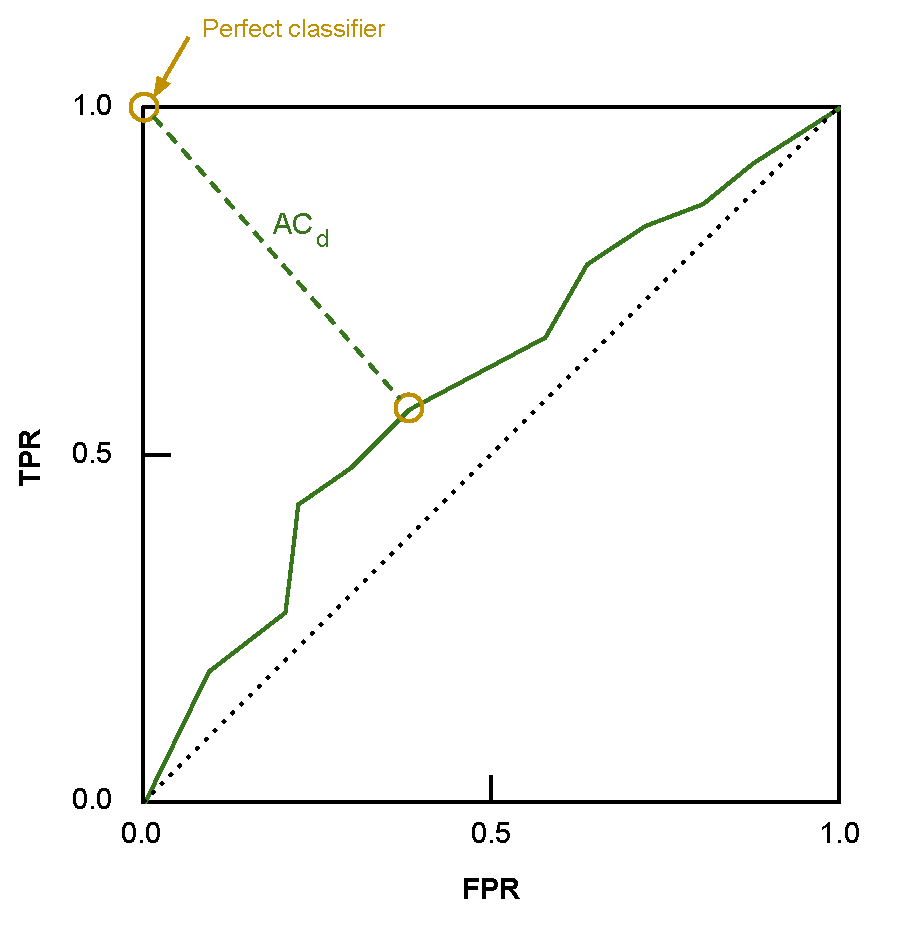
\includegraphics[scale=0.7]{images/roc.pdf}
\caption{ROC (receiving operator characteristics) curve. The $AC_d$ is the distance from a classifier's performance to that of a perfect classifier.}
\label{fig:roc}
\end{figure}

We still lack a single measure that could be used for ranking different classifiers. Since a perfect classifier is the point (0,1) on the ROC curve, we can rank the classifiers based on their distance to that point. Euclidean distance is defined as
\begin{equation}
\text{AC}_d = \sqrt{W \cdot (1 - \text{TPR})^2 + (1 - W) \cdot \text{FPR}^2}, \label{eq:acd}
\end{equation}
where the parameter $W \in [0,1]$ assigns relative importance to false positives and false negatives. The value of $\text{AC}_d$ ranges from 0 for a perfect classifier to $\sqrt{2}$ for a completely incorrect one. \cite{Hamilton12}

To summarize, the parameter selection process goes like this:
\begin{enumerate}
\item{Get parameters values one by one from the grid of available values}
\item{Calculate performance using cross validation and $\text{AC}_d$ as performance measure}
\item{Choose the parameters values with the best performance (highest accuracy or lowest $\text{AC}_d$)}
\end{enumerate}

\subsection{Computational Performance}
Computational performance is not one of the key concerns of this thesis but it is still worth reviewing the possible bottlenecks and ways to improve performance. Not only can the amount of data be huge in CEP, but also the latency with which it is moving should be minimal. That said, our system is of no use if it cannot keep up with new sensor data coming in.

At the core of our system is the Esper CEP Engine which, according to its documentation \cite{EsperReference}, can manage over 500,000 events per second on a dual-core CPU 2 GHz processor with engine latency being less than 3 microseconds on average. The processor on our own test machine is a quad-core CPU 2.5 GHz processor so the performance should be at least at the same level.

It is important to note that training the model does not need to be real-time. In a real-life application the model is trained with regular intervals as a background process. While a new model is being trained, the old model can continue predicting. When the new model is ready, the old model is replaced with it. For example, in our test house this could be done once a month when the indoor air conditions have changed because of, for instance, seasonal changes in the weather.

The prediction phase, in turn, has to be fast as new measurements are coming in all the time. With our DTW and kNN model the prediction includes calculating the DTW distance with each of the training vectors and then selecting \emph{k} closest ones. With our Wavelet and SVM model the prediction phase consists of the Haar Wavelet transform that produces a feature vector and support vector evaluation that classifies the feature vector.

Our computation performance tests evaluate the models' time complexity with respect to window sizes and the number of testing samples. Also the average execution times for classifying a single instance are measured.





\clearpage

\chapter{Implementation and Experiments}
\section{Case Study}
\subsection{ASTEKA Project}
A member of the MMEA project, the research group of Environmental Informatics at the University of Eastern Finland (Kuopio campus) has a project called ASTEKA. The project aims at commercializing a monitoring system of living health and energy efficiency. \cite{Asteka10} Basically, the project equips houses with sensors that provide informative online data presentations for the resident of the house. By monitoring different variables, such as energy consumption and $CO_2$ levels, the house or the resident could adjust the control variables accordingly. 

Their first pilot was introduced at a living fare in Kuopio in the summer of 2010. The pilot originally consisted of 11 houses each of which has sensors ranging from $CO_2$ concentration and temperature to electricity and water consumption. The web interface of the pilot shows daily, weekly and monthly consumption statistics and charts which can be used to improve energy efficiency. \cite{Asteka10} For example, one can easily notice whether the sudden peak in electricity consumption is caused by falling outside temperature or excessive oven usage.


\subsection{Test House and Sensors}
In this thesis I use data from one of the pilot houses. The house has three floors and sensors in all of them. The layout of the first floor is presented in Figure~\ref{fig:floor1}. The squares with numbers in them are sensor units which are listed in Table~\ref{table:floor1}.

\begin{figure}[here]
\centering
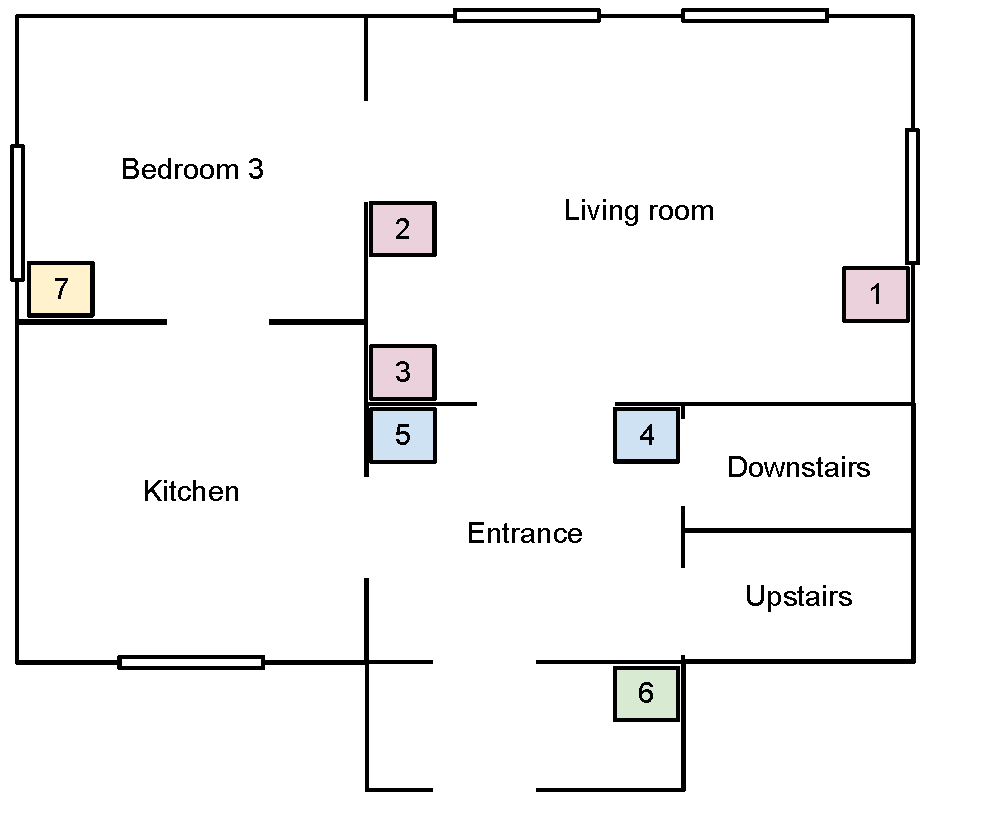
\includegraphics[scale=0.7]{images/keskikerros.pdf}
\caption{Layout of the first floor and the locations of the sensor units.}
\label{fig:floor1}
\end{figure}

The second floor, which has only 2 sensor units, is shown in Figure~\ref{fig:floor2} and its sensors are listed in Table~\ref{table:floor2}. Both the two sensors in the second floor are located in bedrooms. However, bedroom 3 serves as a guest room and thus is empty most of the time, which should be detected in the data easily.

\begin{figure}[here]
\centering
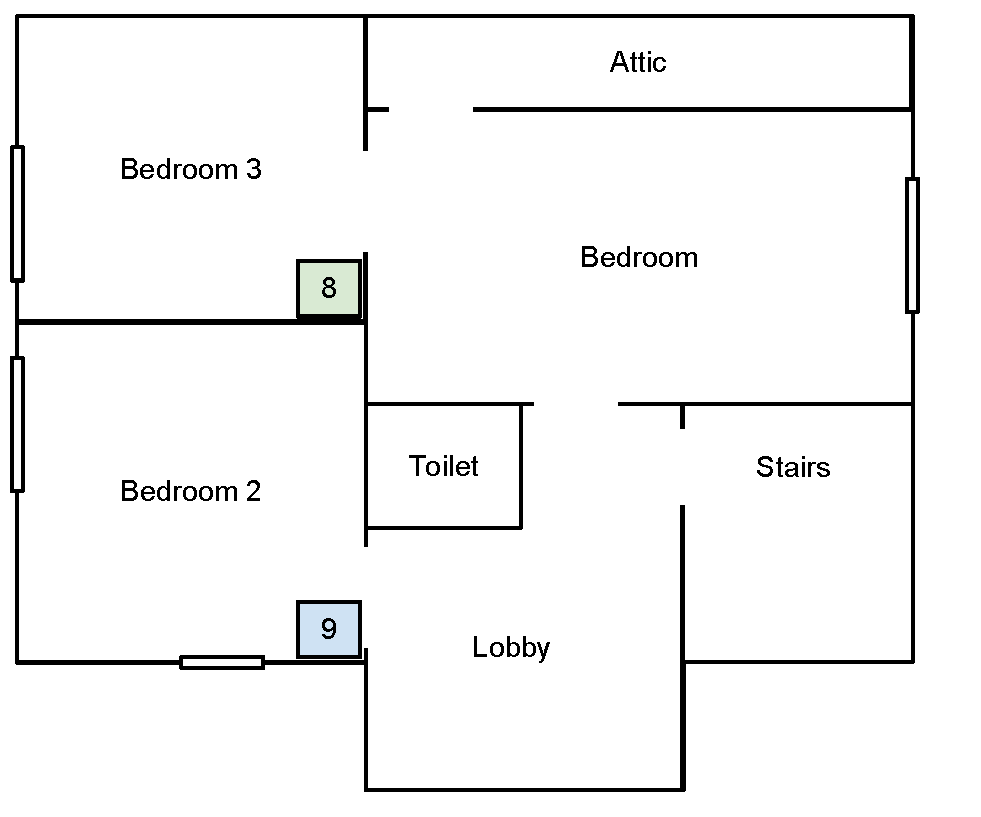
\includegraphics[scale=0.7]{images/ylakerta.pdf}
\caption{Layout of the second floor and the locations of the sensor units.}
\label{fig:floor2}
\end{figure}

In the basement most of the sensors are located in the boiler room which is a well isolated space with no windows. The layout of the basement is presented in Figure~\ref{fig:basement}. The listing of the sensors in the basement is shown in Table~\ref{table:basement}. An interesting detail in the basement is how the sensor unit 10 with humidity and temperature sensors is placed near the showers and the sauna. This should definitely be shown somehow in the data from these sensors.

\begin{figure}[here]
\centering
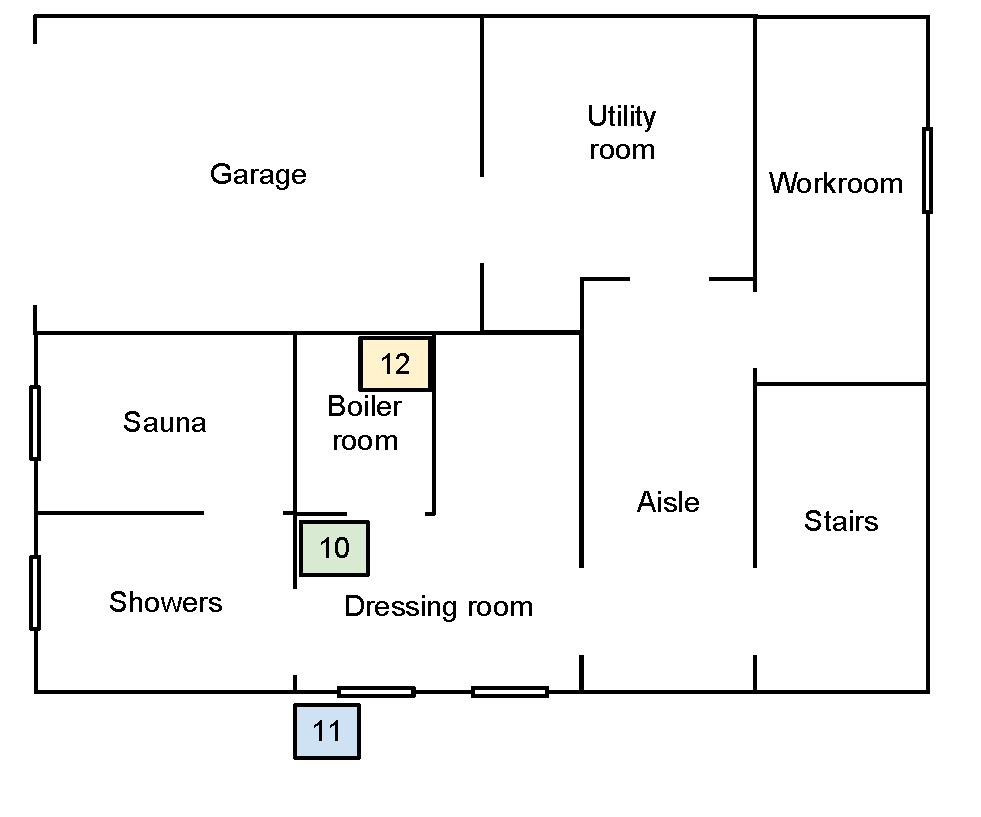
\includegraphics[scale=0.7]{images/kellari.pdf}
\caption{Layout of the basement and the locations of the sensor units.}
\label{fig:basement}
\end{figure}



\begin{table}
  \caption{Sensors in the first floor of the test house} 
  \begin{tabular}{l | l | l | l | c}
    \multicolumn{4}{l}{\textbf{First floor}} \\
    \hline
   	\textbf{Room} & \textbf{Group} & \textbf{Sensor ID} & \textbf{Variable} & \textbf{Unit} \\
    \hline
    Living room & 1 & 51 & Temperature & $^\circ C$ \\
    \hline
    Living room & 2 & 52 & $CO$ & ppm \\
    \hline
    Living room & 3 & 815 & PIR & ON/OFF \\
      &  & 815 & Humidity & \%RH \\
      &  & 817 & Temperature & $^\circ C$ \\
      &  & 818 & $CO_2$ OH & ppm \\
    \hline
    Inner entrance & 4 & 53 & Temperature ET & $^\circ C$ \\
      &  & 54 & Humidity ET & \%RH \\
      &  & 55 & $CO_2$ & ppm \\
      &  & 60 & Electricity & Wh \\
    \hline
    Inner entrance & 5 & 844 & Small particles & count / $ft^3$ \\
     & & 845 & Large particles & count / $ft^3$ \\
    \hline
    Outer entrance & 6 & 56 & Diff Pressure & Pa \\
    \hline
    Bedroom 3 & 7 & 650 & Temperature & $^\circ C$ \\
     & & 651 & Humidity & \%RH \\
     & & 652 & $CO_2$ & ppm \\
     & & 789 & VOC & ppm \\
  \end{tabular}
  \label{table:floor1}
\end{table}

\begin{table}
  \caption{Sensors in the second floor of the test house} 
  \begin{tabular}{l | l | l | l | c}
    \multicolumn{4}{l}{\textbf{Second floor}} \\
    \hline
   	\textbf{Room} & \textbf{Group} & \textbf{Sensor ID} & \textbf{Variable} & \textbf{Unit} \\
    \hline
    Bedroom 1 & 8 & 644 & Humidity & \%RH \\
     & & 645 & Temperature & $^\circ C$ \\
     & & 646 & $CO_2$ & ppm \\
    \hline
    Bedroom 2 & 9 & 647 & Humidity & \%RH \\
     & & 648 & Temperature & $^\circ C$ \\
     & & 649 & $CO_2$ & ppm \\
    \hline
  \end{tabular}
  \label{table:floor2}
\end{table}


\begin{table}
  \caption{Sensors in the basement of the test house} 
  \begin{tabular}{l | l | l | l | c}
    \multicolumn{4}{l}{\textbf{Basement}} \\
    \hline
   	\textbf{Room} & \textbf{Group} & \textbf{Sensor ID} & \textbf{Variable} & \textbf{Unit} \\
    \hline
    Dressing room & 10 & 57 & Humidity & \%RH \\
     & & 58 & Temperature & $^\circ C$ \\
     & & 59 & $CO_2$ & ppm \\
    \hline
    Outside & 11 & 772 & Temperature & $^\circ C$ \\
    \hline
    Boiler room & 12 & 62 & Water & $m^3$ \\
    & & 773 & Floor heating outgoing water & $^\circ C$ \\
    & & 775 & Floor heating & $^\circ C$ \\
    & & 776 & L1 indoor temperature, incoming & $^\circ C$ \\
    & & 777 & Used water & $^\circ C$ \\
    & & 778 & Variable & $^\circ C$ \\
    & & 779 & Radiator outgoing water & $^\circ C$ \\
    & & 783 & Hot water & \% \\
    & & 784 & Radiator indoor temperature & $^\circ C$ \\
    & & 785 & District heating incoming temperature & $^\circ C$ \\
    & & 786 & District heating return temperature & $^\circ C$ \\
    & & 787 & District heating energy & kWh \\
    & & 788 & District heating water flux & $m^3$ \\
  \end{tabular}
  \label{table:basement}
\end{table}

\subsection{Test Data}
The data from ASTEKA server is available via a Java library. The library allows one to specify two dates and it downloads two types of files, sensor files and measurement files. The sensor files are of the following form:

\begin{description}
\item[Filename:]{sensors8\_11.txt}
\item[Header:]{SensorID:int; name:varchar(100)}
\item[Example line:]{51;Temperature Fileplace (Har 1)}
\end{description}

The file name contains to identification numbers: the former is a house ID and the latter is sensor group ID. The header line specifies the columns used in the file but since they are similar in each sensor file, they do not need to be read. The example line shows that the columns are separated by a semicolon.

The measurement files are of the following form:

\begin{description}
\item[Filename:]{measurements8\_11.txt}
\item[Header:]{unixtime(BIGINT); ID\_8\_11\_51(DOUBLE), ID\_8\_11\_52(DOUBLE); ...}
\item[Example line:]{1356998401;21.0253;0.0032; ...}
\end{description}


Like the sensor file names, the measurement file names contain a house ID and a sensor group ID. Again, the header line specifies the columns found in the file. The first column is always an Unix timestamp which tells how many seconds have passed since 1.1.1970 until the the measurement was made. The rest of the columns specify the IDs and the types of the values the sensor is emitting. The numbers in pattern \emph{ID\_8\_11\_51} are house ID, sensor group ID and sensor ID, respectively. After that there is the variable type specified.

The complex events we are trying to detect are defined in Chapter 4.4.



\section{Implementation}

A test version of the predictive event processing network was created with Java programming language. Java was chosen because of several reasons:
\begin{itemize}
\item{Java is the main development language of MMEA platform}
\item{Esper CEP Engine provides easy-to-use API for Java}
\item{Test data is available via a Java library}
\item{The performance of Java is sufficient}
\end{itemize}

Unlike the MMEA platform that uses PostgreSQL and Amazon S3 as database solutions, I have chosen MySQL as my development database because I am more familiar with it. I use an ORM (Object-relational mapping) layer called Hibernate between my program and the database. Thus, using a different database solution is only a matter of changing the database adapter from MySQL to something else in the Hibernate configuration file.

The goal of this chapter is to present a framework for integrating a predictive component alongside with a Event Processing Network. The approach is quite technical meaning that anyone with adequate skills in Java and Esper could replicate the system and improve it with their own expertise.

\subsection{Data Structures}
The test data is mapped into four Java classes that directly correspond to tables in my own MySQL database. This mapping is done with Hibernate library, which allows the programmer to annotate, that is, add table specifications Java classes. Then, Hibernate creates the database schema using these annotations. In the following I will describe these four classes in a compact form stating only the name of the class and parameter types and names. 

First class represents the house we are dealing with:
\begin{Verbatim}[xleftmargin=1.5em]
public class House {
	int houseId;
	String name;
	Map<Integer, Sensor> sensors;
	Set<MeasurementUnit> units;
},
\end{Verbatim}
where, the parameter \emph{sensors} is a map from sensor IDs to sensor objects and the parameter \emph{units} contains all the measurement events from that house.

The second class represents a single sensor:
\begin{Verbatim}[xleftmargin=1.5em]
public class Sensor {
	House house;
	int sensorId;
	String name;
}
\end{Verbatim}

The third class represents a single measurement event which, in turn, may contain multiple measurement values from different sensors:
\begin{Verbatim}[xleftmargin=1.5em]
public class MeasurementUnit implements TimedEvent {
	House house;
	Date timestamp;
	Set<MeasurementValue> values;
}
\end{Verbatim}

The last class represents a single measurement value:

\begin{Verbatim}[xleftmargin=1.5em]
public class MeasurementValue {
	Sensor sensor;
	MeasurementUnit measurementUnit;
	double value;
}
\end{Verbatim}

As can be seen, \emph{MeasurementUnit} class implements an interface called \emph{TimedEvent} which is a common interface for all events in this thesis. It requires the class to have a timestamp property that can be used to mark the occurrence of an event in the time space. Objects from the class \emph{MeasurementUnit} are the most important ones because the event source emits them to the CEP engine. The processing of these events is described in the following chapter.



\subsection{Predictive Event Processing Network}
The Predictive Event Processing Network (PEPN) is a separate network as described in Chapter 3.2. In this thesis I have made the separation so clear that the two networks even have their own Esper engines. In some publications (e.g. \cite{Fulop12}) the PEPN just integrates into the EPN's engine but in this thesis' approach some Event Processing Agents (EPAs) connect to both networks and transfer data between them. 

The structure of the Event Processing Network (EPN) defines which Complex Events the system captures and it depends on the phenomenon in question. However, the structure of the PEPN is completely independent of the EPN meaning that the framework presented here should, in theory, work for each Complex Event type that is predictable with the predictive models used here. The phenomenon-specific EPNs (and its EPAs) will be defined in experimental design chapter. The framework for PEPN is presented in Figure~\ref{fig:pepn}.

\begin{sidewaysfigure}[here]
\centering
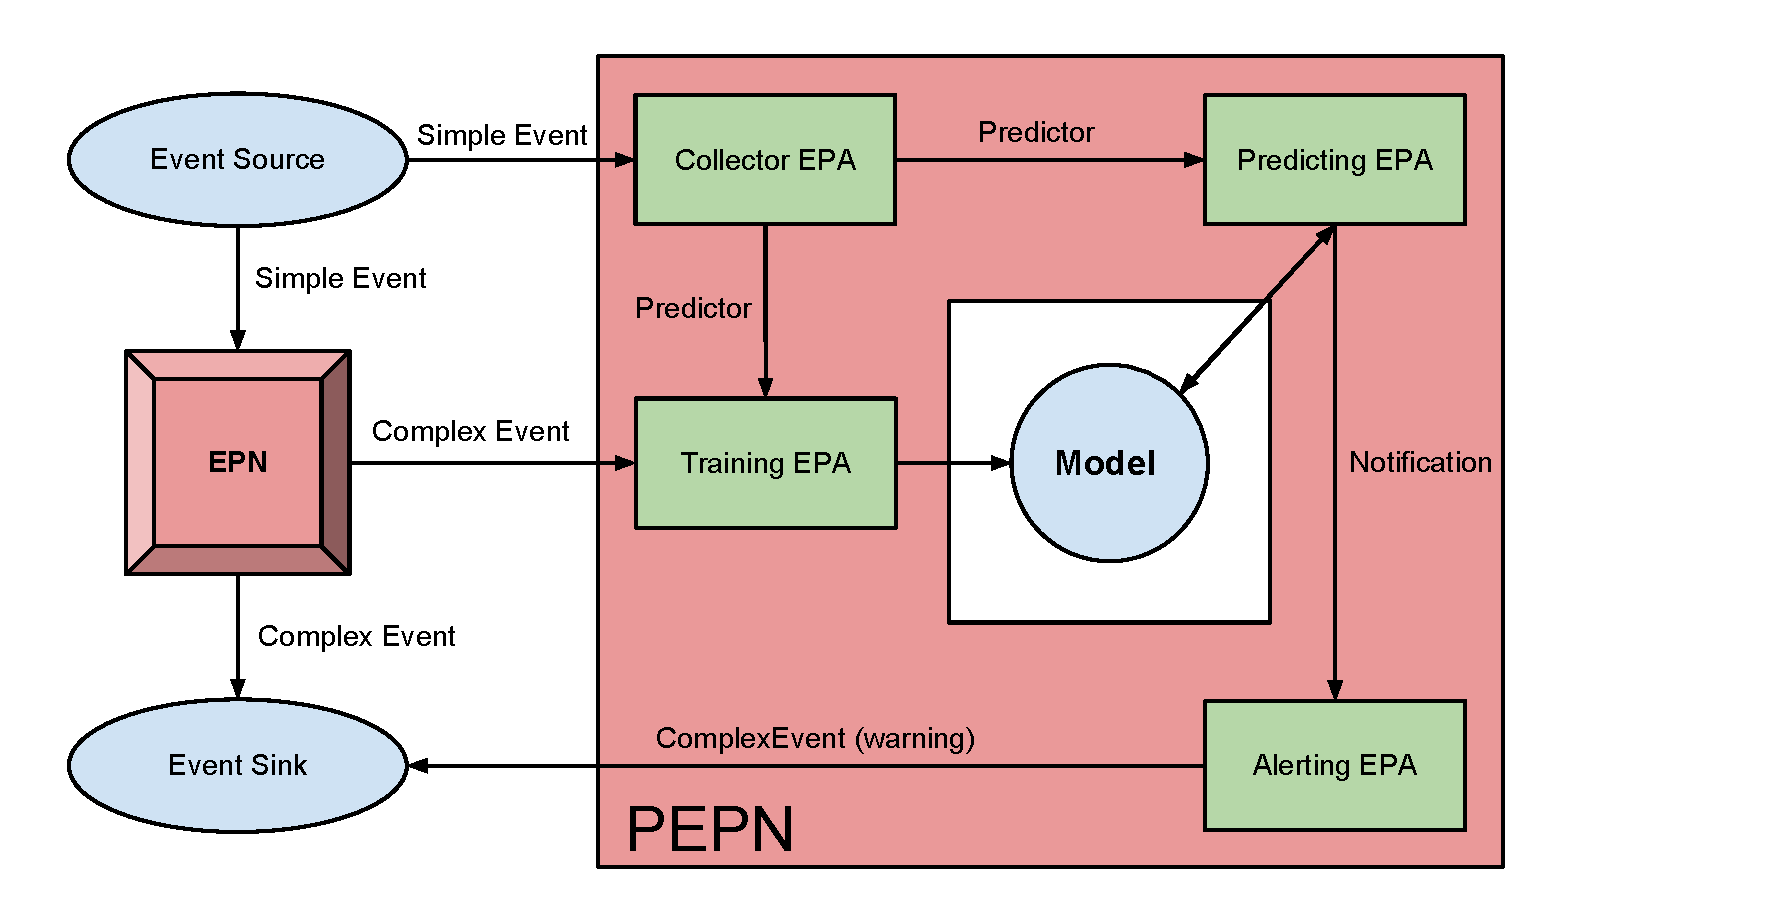
\includegraphics[scale=0.7]{images/epn.pdf}
\caption{Event Processing Network (EPN) and Predictive Event Processing Network.}
\label{fig:pepn}
\end{sidewaysfigure}


On the left side of the figure there is the EPN that attaches to the event sources, processes the data and outputs a Primary Complex Event (PCE) to the event sink. In this concept we don't place any restrictions for neither the format of input data nor the structure of the data processing. However, the output of the EPN must be unique, that is, only one type of output is allowed. Thus, the output can be formalized as the following Java class
\begin{Verbatim}[xleftmargin=1.5em]
public class ComplexEvent {
	Date timestamp;
	String message;
},
\end{Verbatim}
where the timestamp marks the time when the complex event takes place and the message contains relevant information about the event type that can be shown to the user when the event happens. 

In Esper an event listener specifies an EPL and implements the interface
\begin{Verbatim}[xleftmargin=1.5em]
public interface UpdateListener {
	public void update(EventBean[] newEvents, EventBean[] oldEvents);
}
\end{Verbatim}

When the EPL is triggered, the \emph{update} method is called and the events entering the window are given in \emph{newEvents} array while the events leaving the window can be found from \emph{oldEvents}. \cite{EsperReference} In this thesis, an Event Processing Agent (EPA) is required to provide an EPL clause and to implement the interface above.


The Predictive Event Processing Network (PEPN) has four different Event EPAs that collect and preprocess the incoming data. 

\emph{CollectorEpa} listens to EPN's event sources and collects predictor vectors for training and predicting phases. Its EPL is of the form
\begin{Verbatim}[xleftmargin=1.5em]
SELECT 
	value('<sensorId>').value as value, 
	time 
FROM 
	MeasurementUnit.win:time(<windowLength>)
OUTPUT SNAPSHOT
	every <windowDifference>
\end{Verbatim} 

Here the first select item uses \emph{MeasurementUnit}'s getter for measurement values and then uses its getter for value. The clause defines a sliding window whose length is given as a parameter \emph{windowLength} for the EPL. The last part, \emph{output snapshot every windowDifference}, triggers the \emph{update} method with the given time interval. Then, Esper's pull API allows us to iterate through the window's contents. \cite{EsperReference} This EPL creates the predictor vectors that are then consumed by other EPAs.

Next, as can been from Figure~\ref{fig:pepn}, \emph{TrainingEpa} and \emph{PredictingEpa} use the predictors emitted by \emph{CollectorEpa} as their input. In this case, the predictors are instances of the class \emph{MeasurementVector}, which is of the following form
\begin{Verbatim}[xleftmargin=1.5em]
public class MeasurementVector implements TimedEvent, LabeledSample {
	Date timestamp;
	Date endTimestamp;
	List<Double> values;
	Label label;
},
\end{Verbatim}
where values list contains the measurement values between \emph{timestamp} and \emph{endTimestamp}. \emph{MeasurementVector} is a time series which we are trying to classify. It implements the interface \emph{LabeledSample} which requires it to have a \emph{Label} property. The \emph{TrainingEpa} listens also to the EPN's \emph{ComplexEvent}s and its EPL is as follows
\begin{Verbatim}[xleftmargin=1.5em]
SELECT predictor.*
	FROM pattern[
		every predictor=MeasurementVector 
		-> (timer:interval(<waitingTime>) 
		-> (timer:interval(<eventTime>) and <Negation>c=ComplexEvent))
	],
\end{Verbatim} 
which needs a bit clarification. The pattern in the EPL first looks for a \emph{MeasurementVector} event from \emph{CollectorEPA}. The \emph{every} keyword initiates this lookup on each event. When an event is found, the first timer waits an interval of length \emph{waitingTime}. Then, the second interval looks for an interval of length \emph{eventTime} during which a \emph{ComplexEvent} is found. The variable \emph{Negation} is either empty or ``not '', which allows us to detect both positive and negative instances. For this purpose, we can define two \emph{TrainingEPA}s: one for positive instances with \emph{Negation} being empty and one for negative instances with \emph{Negation} set to ``not ''.

Now the \emph{TrainingEPA} collects the predictors but the next step is to decide when to perform the actual training process. For this purpose a \emph{TrainingInvokerEPA}, which is not shown in the pictures as it ``lives'' inside the \emph{TrainingEPA}. It declares an EPL of the form

\begin{Verbatim}[xleftmargin=1.5em]
SELECT 
	* 
FROM 
	pattern[every timer:interval(<trainingInterval>)],
\end{Verbatim} 
which is triggered automatically based on the time variable \emph{trainingInterval}. Then, the \emph{update} is called and it executes the training of the model.

Like the \emph{TrainingEpa}s, \emph{Predictor}EPA is fed with predictors (\emph{MeasurementVectors}) as shown in Figure~\ref{fig:pepn}. Both \emph{TrainingEPA}s and \emph{PredictorEPA} communicate directly with a specific model class that extends an abstract \emph{Model} class. Sub-classes of Model implement a certain model, in this case either a DTW and kNN-based one or a Wavelet and SVM-based one. The Model collects labeled predictors from \emph{TrainingEPA}s until its \emph{train()} method is called.

The \emph{PredictorEpa}, in turn, calls the Model's classify(\emph{MeasurementVector})-method, which returns the label for the given predictor. If the instance is classified as positive, a notification event is sent to the PEPN, which is then captured by \emph{AlertingEPA}. Then, the \emph{AlertingEPA} builds a \emph{ComplexEvent} and outputs it to the original EPN. In this way, the PEPN creates a warning for the EPN.


\subsection{Data Flow and Performance Tuning}
The event source reads a block of data from the database and sends it to both EPN and PEPN as can be seen in Figure~\ref{fig:pepn}. Then, the event processing networks process the data with their own EPAs. Without giving any thought to concurrency, this approach faces the problem of blocking as the event source does not start reading new data until the processing of old data is finished. 

To solve this problem we use threads that are kind of lightweight processes. \cite{Java} Unlike actual processes, threads share the same memory space and are actually contained within one process. On a single-core processor the operating system can use time slicing feature to allow threads to execute code almost concurrently. On a multi-core processor the system's capability for concurrent processes enhances significantly.

Our system has four threads: main thread, event source thread, EPN thread and PEPN thread. The last three threads are initialized and started from the main thread. To exchange data between two threads we need a data structure that supports concurrent processing. The data structure should be some kind of queue as the event source fills it with data and the two networks read from it. The Java programming language offers several implementations for concurrent queues. A suitable choice is \emph{LinkedBlockingQueue}, a First-In-First-Out (FIFO) queue, which offers the following methods \cite{Java}
\begin{description}
\item[void put(Object)]{Inserts the specified element into this queue, waiting if necessary for space to become available.}
\item[void take()]{Retrieves and removes the head of this queue, waiting if necessary until an element becomes available.}
\end{description}

In our system there are two of these queues: one between event source and EPN and one between event source and PEPN. Now the event source can read a batch of data from the database and call \emph{put(e)} for each element. Then, both networks, being in an infinite loop calling \emph{take()}, start processing data as soon as it becomes available.




\subsection{Machine Learning Libraries}
In this thesis I use two ready-made machine learning libraries: Java Machine Learning Library (Java-ML) \cite{javaml} and Weka 3: Data Mining Software in Java \cite{weka}. This approach allows me to concentrate not on the implementation of the algorithms but on the proper use of the methods. More importantly, the algorithms used in the libraries have already been optimized and tested properly by machine learning experts.

Java-ML contains an implementations for Dynamic Time Warping (DTW) and k-Nearest Neighbor (kNN) algorithms. Together with Java-ML's \emph{CrossValidation} class, it is fairly easy to choose optimal parameter values. This algorithm, however, lacks the possibility of receiving intermediate results. For this reason I created an implementation by following the pseudo-code from section 3.6.1.

For a given set of parameters, the cross validation algorithm returns an instance of the class \emph{PerformanceMeasure}, which contains the variables TP, FP, TN and FN. From these I calculate the value for the $AC_d$ as described in (109)-(116). Then, the set of parameters with the lowest $AC_d$ is chosen.

Java-ML has a wrapper for LibSVM which is an efficient Support Vector Machine library \cite{libsvm}. The interface provides Java classes that call the fast underlying C implementations. LibSVM comes with a class called \emph{GridSearch}, which performs the grid search for parameters $C$ and $\gamma$ as described in Chapter 3.5.7. Again, I implemented the grid search in order to receive intermediate results.

In this thesis the Weka library is used to perform the wavelet transform and it supports the Discrete Haar Wavelet Transform. The conversion between Weka and Java-ML data formats is easy as their \emph{Instance} classes provide getter and setter method for plain double arrays that contain the vector data.







\section{MMEA Platform Architechture}

\subsection{Technology Overview}
MMEA platform is designed to use Service Oriented Architecture (SOA) which means that different processes and components are implemented as independent and flexible services. These loosely coupled services use one another through open interfaces. This architecture pattern facilitates the integration of new components into the system and allows the services to be distributed into several physical machines. 

The MMEA platform runs on the Amazon Web Services (AWS) cloud which consists of Amazon Elastic Compute Cloud (EC2) and Amazon Simple Storage Service (S3). The former is a cloud computing platform where users can install virtual servers called instances and the latter is a cloud storage service where users can store application data through web services. Both services are billed as a pay-as-you-go service which means that users can scale the computing resources whenever needed and pay only for the resources used. By using a cloud-based approach the costs and the amount of maintenance of physical servers can be eliminated.

The SOA principle in MMEA is implemented using an open-source Enterprise Service Bus (ESB) from WSO2 software company. WSO2 ESB is a lightweight and high performance integration layer between different services. It uses Java Message Service (JMS) for exchanging messages between distributed and loosely-coupled services. The ESB integrates the five other MMEA layers
\begin{description}
\item[Sensor Layer]{Connects to sensor systems with sensor-specific adapters}
\item[Storage Layer]{Stores data into a database and loads data from it}
\item[Model Layer]{Runs computations based on problem-specific models}
\item[Control Layer]{Provides interfaces for monitoring and managing the system}
\item[Presentation Layer]{Provides data for external applications}
\end{description}
These layers are shown in Figure~\ref{fig:mmea}.

\begin{figure}[here]
\centering
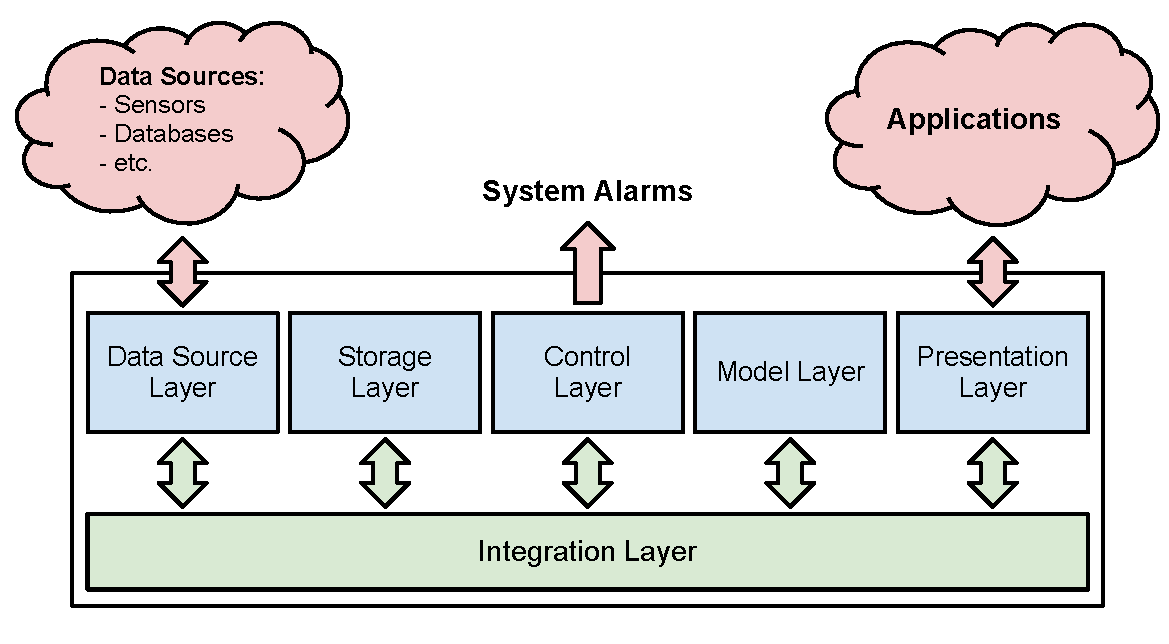
\includegraphics[scale=0.7]{images/mmea.pdf}
\caption{MMEA Platform layers.}
\label{fig:mmea}
\end{figure}

At the core of the application layer there is a component called publish/subscribe which works over SOAP, an XML-based web service for messaging. External applications can publish their data feed and send their new data into the MMEA platform. Other parties can subscribe to these feeds and utilize the data in their processes, such as alarm services.

The MMEA platform has its own data format called MMEA Bus Message, which is an XML-based message format. It has a separate XML schema for common platform messages, sensor observation messages, forecast messages and complex event messages. For example, a sensor observation message contains information about the producer and the location of the sensor, as well as the measurand and the observed value. The sensor layer adapters define XSLT (Extensible Stylesheet Language Transformations) transformations from the producers' data formats into the MMEA Message Bus format.



\subsection{Integrating the Predictive Component}
The predictive complex event processing network must be integrated to the existing platform architecture so that the platform remains easily maintainable. As can be seen from the layer descriptions in the previous chapter, the MMEA platform has a model layer, which is used to run computations on problem-specific models. The predictive component can be integrated to this layer and run on the same physical computational cluster.

Another, and perhaps a better way to integrate the predictive component is to create an external application that is loosely coupled with the MMEA platform. In this approach the CEP engine and the predictive component are running on separate machine and use the publish/subscribe method provided by MMEA platform. Predictive component subscribes to feed that provides new sensor data. Then, having analyzed the data, it can publish the complex events, that is, the alarms back to the MMEA platform.






\section{Experimental Design}
In this section I first define the complex events that are predicted in the experimental part. Then, I describe some test settings that are employed in this thesis.
\subsection{Complex Event Definitions}
A simple Complex Event is a sensor value exceeding a certain predefined limit for a certain time. For each sensor type (temperature, $CO_2$, etc.) we can write a Java classes
\begin{Verbatim}[xleftmargin=1.5em]
public class ValueClassification {
	Set<Sensor> sensors;
	List<ValueClassificationLimit> limits;
}
\end{Verbatim}
and
\begin{Verbatim}[xleftmargin=1.5em]
public class ValueClassificationLimit {
	String name;
	double limit;
	int level;
}
\end{Verbatim}

The former represents a classification scale for one type of sensors and the latter is an actual limit. The \emph{limit} attribute is the lower bound limit for an measurement value to belong to that class. The \emph{level} attribute gets integer values beginning from 0 and can be used to display only \emph{ClassificationEvent}s beginning from a given level. It can be thought as severity of the event.

Now we can further define a complex event that rises from exceeding a classification limit
\begin{Verbatim}[xleftmargin=1.5em]
public class ClassificationEvent extends ComplexEvent {
	Date timestamp;
	Sensor sensor;
	ValueClassificationLimit limit;
	String length;
},
\end{Verbatim}
which is a sub-class of \emph{ComplexEvent}. It contains all the relevant information about the event: the timestamp of the event, the sensor that caused the event, the limit value which was exceeded and the length of time window that triggered the event. 

An Event Processing Agent (EPA) called \emph{ClassificationEPA} loads the classification limits from the database and builds the EPL clauses that detect the classification events. Let's say we have a sensor with \emph{SensorID} 50 and the complex event happens when the measurement value exceeds the value of 100 for 20 minutes. Then, the following EPL detects the classification event of level 2 and builds a complex event that is sent to the CEP engine
\begin{Verbatim}[xleftmargin=1.5em]
INSERT INTO
	ClassificationEvent
SELECT 
	unit.timestamp AS time,
	unit.value('50').sensor AS value, 
	2 AS minLevel,
	'20 min' AS windowLength 
FROM
	pattern[
		every (timer:interval(20 min) 
		and unit=MeasurementUnit(value('50').value > 100))		
	]	
\end{Verbatim}

Next, we need to specify the limits for each measurand. For $CO_2$ and VOC (Volatile Organic Compounds) we can use the indoor air quality classes defined by the Finnish Indoor Air Society. \cite{sisailmaluokitus08} The classification supports the evaluation of construction and renovation processes from the air quality's point of view.

Indoor Air Society has defined three classes, S1, S2 and S3, which describe the indoor air quality in the following way
\begin{description}
\item[S1: Individual]{Excellent indoor air quality. No detectable odors or sources of pollutants. Controllable temperatures with no overheating.}
\item[S2: Good]{Good indoor air quality. No disruptive odors or sources of pollutants. No detectable breeze but overheating possible during summer.}
\item[S3: Satisfactory]{Air quality and temperature conditions fulfill construction requirements.}
\end{description}

For $CO_2$ and VOC the class limits are shown in Table~\ref{table:voc_co2_quality}. For VOC the corresponding values from our sensor are shown in parentheses.


\begin{table}[h!]
\begin{center}
  \caption{Air quality classifications for $CO_2$ and VOC.} 
  \begin{tabular}{c|c|c}
  	Class & $CO_2$ (ppm) & VOC ($\mu g/m^3$) \\
	\hline
	S1 & 0-700 & 0-200 (0-10) \\
	S2 & 700-900 & 200-300 (10-20) \\
	S3 & 900-1200 & 300-600 (20-30) \\
	S4 & >1200 & >600 (>30) 
  \end{tabular}
  \label{table:voc_co2_quality}
\end{center}
\end{table}

The particle detector counts the number of small particles in two size groups: particles with diameter between 1 $\mu$m and 5 $\mu$m and particles with diameter greater than 5 $\mu$m. The former group consists of fine dust, smoke, mold and bacteria while the latter is made of coarse dust, pollen and dust mite casings. The detector in our test house, Dylos DC1100, is calibrated to detect particles half the size mentioned before, that is 0.5 $\mu$m and 2.5 $\mu$m.

On the backside of the particle detector device, there is an air quality chart defined for the smaller particle size. This classification is presented in Table~\ref{table:particles}. The first column defines the classification in our system. The other two columns have been read from the device's backside. In the range 0-300 three classes, excellent, very good and good, have been combined into one class, PC1.

\begin{table}[h!]
\begin{center}
  \caption{Air quality classifications for $CO_2$ and VOC.} 
  \begin{tabular}{c|c|c}
  	Class & Particle count & Description \\
	\hline
	PC1 & 0-300 & Good/Excellent \\
	PC2 & 300-1050 & Fair \\
	PC3 & 1050-3000 & Poor \\
	PC4 & >3000 & Very Poor
  \end{tabular}
  \label{table:particles}
\end{center}
\end{table}


Similar classifications can be defined for heating and electricity consumption by determining the class ranges from the historical data. In more detail, the ranges were chosen to cover most often occurring peak values during the turning of the season. In this way, the most relevant complex events could be created for each time period (time of year). The classes are presented in table~\ref{table:particles}

\begin{table}[h!]
\begin{center}
  \caption{Classifications for electricity and heating.} 
  \begin{tabular}{c|c|c|c}
  	Electricity Class & Consumption (kW) & Heating Class & Consumption (kW) \\
	\hline
	EC1 & 0-2 & HC1 & 0-10 \\
	EC2 & 2-3 & HC2 & 10-20 \\
	EC3 & 4-5 & HC3 & 20-30 \\
	EC4 & >5 & HC4 & >30			
  \end{tabular}
  \label{table:particles}
\end{center}
\end{table}


%\subsubsection*{Multiple Classification Event}
%In many real-life applications a single parameter exceeding a limit value does not necessarily mean anything. However, two or three sensors showing increased levels may indicate there is something seriously


\subsection{Selecting Parameters and Running the Tests}

Two different prediction schemes are tested. The first starts with a training period of \emph{trainingDays} days and continues with a series of testing periods of length \emph{testingDays} for the rest of the data. The latter first trains the model with \emph{trainingDays} days and then runs \emph{testingBatches} single tests of length \emph{testingDays}. This is process is then repeated until the data ends. 

A long data set may show radical changes in indoor air quality conditions. If that is the case, then the second testing scheme which trains the model more often should perform better. This is one of the main focus points of the experimental section.

Our data collection phase has five different constants which were introduced in the previous chapters. A clarification for the first three parameters was shown in Figure 2.

\begin{description}
\item[windowLength]{Length of measurement vector that is used as a predictor.}
\item[waitingInterval]{Part of the prediction horizon that is ignored.}
\item[eventInterval]{Part of the prediction horizon which determines the class of the predictor depending whether or not a complex event happens within it.}
\item[windowDifference]{Determines how often a new predictor is created. Difference between two predictors' start points.}
\item[exceedTime]{Determines the minimum time interval that triggers a classification event, that is, a sensor value exceeds a certain limit.}
\end{description}

Depending on the sensor, a certain combination of these parameters works better. For each sensor, each parameter is given a set of possible values. Then, the tests are run for each combination of parameters and the best combination is selected. The possible values are selected by inspecting the time series graph.

In addition to these parameters, the prediction models have parameters of their own, too. Each training process is run as a grid search and the best combination of the model parameters is used in the testing phase. For DTW and kNN based model those parameters are
\begin{description}
\item[radius]{Maximum deviation from the optimal path in DTW (see Chapter 3.4.2). Possible values: 5 and 50.}
\item[k]{The only parameter for k-Nearest Neighbour algorithm (see Chapter 3.4.3). Possible values: 3, 7 and 15.}
\end{description}

The selected possible values produce a total of $2 \cdot 3 = 6$ combinations for the grid search. The smaller the \emph{radius} for DTW is, the less accurate the algorithm is because the allowed deviation from the optimal path is smaller. The value of \emph{k} for kNN determines how sensitive the classifier is to noise; the larger the parameter is, the less sensitive the classifier is to noise \cite{everitt11}.

For SVM the parameter grids were presented in Chapter 3.7.6.
\begin{description}
\item[$\mathbf{\gamma}$]{Parameter for the Gaussian Kernel. $a_0 = 3$}
\item[C]{Soft margin parameter. $C_0 = 5$}
\end{description}

The selected values produce a total of $7 * 6 = 42$ combinations for the grid search.





\clearpage

\chapter{Results}
%\subsection{Class Separability}



\section{Goodness Indicators}
\subsection{Classification With DTW and kNN}
\subsection*{Variable: $CO_2$ Concentration}
The first test is performed with $CO_2$ sensor from the bedroom 1 on the second floor (group 8 and sensor ID 646 in Table 2). The test data is from November 1st, 2012 until February 28th, 2013. One example week from that four month period is shown in Figure~\ref{fig:co2_1}. The classification levels defined in Chapter 4.1 are shown in the figure as well as one missing part that is covered with linear interpolation. For $CO_2$ the minimum level for an alert is set to S2, which is the red line in the picture.

\begin{center}
\begin{figure}[h!]
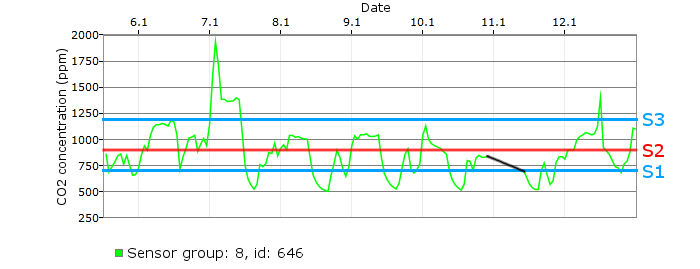
\includegraphics[scale=0.7]{images/co2_1.png}
\caption{Example time series from $CO_2$ sensor. The S1, S2 and S3 mark the classification limits.}
\label{fig:co2_1}
\end{figure}
\end{center}

First, let us investigate the effects of DTW and kNN parameters on the classification results. It is reasonable to suppose that the values of \emph{radius} and \emph{k} should have only a minor effect on the classification results. The time parameters were set to the following values
\begin{itemize}
\item{windowLength: 4 hours}
\item{windowDifference: 1 hour}
\item{waitingInterval: 30 min}
\item{eventInterval: 2 hours}
\item{exceedTime: 30 min}
\end{itemize}

These values mean that a new four-hour predictor vector is created every hour. This predictor is considered positive if the sensor value exceeds the limit value for 30 minutes within two hours after the predictor and a waiting time of 30 minutes.

A 30-day period from November 2012 with a total of 267,524 events was used to test the six parameter combinations. The first 70 \% of the data was used for training and the rest for testing. The classification results are shown in Table~\ref{table:co2_dtwknn_1}.


\begin{table}
  \caption{Results for November 2012 with DTW and kNN model ($W = 0.5$). The definition of ROC distance $AC_d$ is shown in (\ref{eq:acd}). For each row the number of positive samples is $\text{P} = \text{TP} + \text{FN} = 134$ and the number of negative samples is $\text{N} = \text{FP} = \text{TN} = 99$.} 
  \begin{tabular}{ c | c | c | c | c | c | c | c | c | c }
    \hline
   	\textbf{radius} & \textbf{k} & \textbf{TP} & \textbf{FP} & \textbf{TN} & \textbf{FN} & \textbf{TPR} & \textbf{FPR} & \textbf{Accuracy} & $\mathbf{AC_d}$ \\
	\hline
	5 & 3 & 110 & 18 & 81 & 24 & 0.92 & 0.13 & 0.82 & 0.16 \\
	5 & 7 & 103 & 8 & 91 & 31 & 0.77 & 0.060 & 0.83 & 0.17 \\
	5 & 15 & 101 & 9 & 90 & 33 & 0.75 & 0.067 & 0.82 & 0.18 \\
	50 & 3 & 108 & 15 & 84 & 26 & 0.81 & 0.11 & 0.82 & 0.16 \\
	50 & 7 & 102 & 7 & 92 & 32 & 0.76 & 0.052 & 0.83 & 0.17 \\
	50 & 15 & 103 & 6 & 93 & 31 & 0.77 & 0.045 & 0.84 & 0.17 \\
	\hline
  \end{tabular}
  \label{table:co2_dtwknn_1}
\end{table}

As can be seen from the results, the parameters \emph{radius} and \emph{k} do not have much effect on the classifier performance. Thus, the simplest possible model is selected. For the rest of the experiments values $radius = 5$ and $k = 3$ will be used.

Next, we perform the two experiments described in Chapter 4.4.2. The first test trains the model with 14 days of data and then runs tests in batches of 7 days. The second test runs three iterations, each beginning with a training period of 14 days and then three 7-day test batches. The parameters are the same as in the previous test except for the \emph{exceedTime} which is now set to 1 hour.

The results from these experiments are shown in Table~\ref{table:co2_dtwknn_2}. As can be seen from the table, there is no significant difference between constantly updating model and using the the same model for all tests.


\begin{table}
  \caption{DTW and kNN based model. 1: Periodically trained model. 2: Model that is trained only once.} 
  \begin{tabular}{ c | c | c | c | c }
    \hline
   	\textbf{Week} & \textbf{1: Purpose} & \textbf{1: Accuracy} & \textbf{2: Purpose} & \textbf{2: Accuracy} \\
	\hline
	1 & Training & - & Training & - \\
	2 & Training & - & Training & - \\
	3 & Testing & 0.72 & Testing & 0.72 \\
	4 & Testing & 0.81 & Testing & 0.81 \\
	5 & Testing & 0.71 & Testing & 0.71 \\
	6 & Training & - & Testing & 0.75 \\
	7 & Training & - & Testing & 0.86 \\
	8 & Testing & 0.88 & Testing & 0.94 \\
	9 & Testing & 0.91 & Testing & 0.94 \\
	10 & Testing & 0.75 & Testing & 0.75 \\
	11 & Training & - & Testing & 0.84 \\
	12 & Training & - & Testing & 0.86 \\
	13 & Testing & 0.76 & Testing & 0.72 \\
	14 & Testing & 0.81 & Testing & 0.83 \\
	15 & Testing & 0.81 & Testing & 0.84 \\
	\hline
  \end{tabular}
  \label{table:co2_dtwknn_2}
\end{table}

The $CO_2$ consumption seems to be quite easy to predict with this data set because the peaks are quite wide and they occur with constant intervals. The EPN is likely to capture two kinds of complex events: ones that actually precede peaks and ones that are within a peak indicating that the peak will continue.

As of the beginning of April, 2013, the test house was equipped with a mechanical ventilation system which improved the air quality significantly. This change eliminates the periodic increase in $CO_2$ levels we tried to predict in the previous tests. As a comparison, the model was evaluated with four one-week periods from March and April, 2013. These results are shown in Table~\ref{table:co2_dtwknn_3}.

\begin{table}
  \caption{Performance of DTW and kNN based model in the spring of 2013. The mechanical ventilation system was installed in the beginning of April.} 
  \begin{tabular}{ c | c | c | c | c | c | c | c | c | c | c }
    \hline
   	\textbf{Start} & \textbf{End} & \textbf{P} & \textbf{N} & \textbf{TP} & \textbf{FP} & \textbf{TN} & \textbf{FN} & \textbf{TPR} & \textbf{TNR} & \textbf{Accuracy} \\
	\hline
	01.03.13 & 08.03.13 & 42 & 61 & 19 & 1 & 60 & 23 & 0.45 & 0.98 & 0.77 \\
	08.03.13 & 15.03.13 & 17 & 70 & 7 & 1 & 69 & 10 & 0.41 & 0.99 & 0.87 \\
	15.03.13 & 22.03.13 & 11 & 76 & 2 & 2 & 74 & 9 & 0.18 & 0.97 & 0.87 \\
	29.03.13 & 06.04.13 & 32 & 57 & 25 & 0 & 57 & 7 & 0.78 & 1.00 & 0.92 \\
	06.04.13 & 13.04.13 & 2 & 83 & 0 & 3 & 80 & 2 & 0.00 & 0.96 & 0.94 \\
	13.04.13 & 20.04.13 & 2 & 83 & 0 & 2 & 81 & 2 & 0.00 & 0.98 & 0.95 \\
	20.04.13 & 27.04.13 & 2 & 83 & 1 & 1 & 82 & 1 & 0.50 & 0.99 & 0.98 \\
	\hline
  \end{tabular}
  \label{table:co2_dtwknn_3}
\end{table}

As can be seen from the number of positive testing samples in Table~\ref{table:co2_dtwknn_3}, the $CO_2$ levels decreased after the installation of mechanical ventilation system. Or at least the periodic peaks disappeared. The model now struggles with positive sample with \emph{TPR} being much worse than in the previous tests. In the winter the average \emph{TPR} was $0.76$ for the same model.


\subsection*{Variable: VOC}
As a second test variable we are using Volatile Organic Compounds (VOC). The sensor ID is 789 and the group is 7. It is located in a bedroom in the first floor. 

As the last chapter indicated, we would not get much advantage from parameter optimization. Thus, we continue using the same values $k = 3$ and $radius = 5$. A sample week of the data is shown in Figure~\ref{fig:voc_1}.

\begin{center}
\begin{figure}[h!]
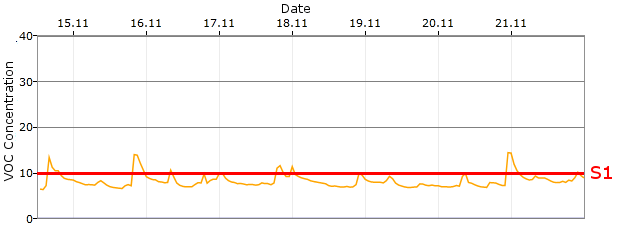
\includegraphics[scale=0.7]{images/voc_1.png}
\caption{VOC concentration.}
\label{fig:voc_1}
\end{figure}
\end{center}

As the figure shows, this time the peaks that exceed the limit value (S1) are much sharper. Thus, we first try to find the optimal time constants. The test data is again from November, 2012.

Two time parameters, \emph{windowDifference} and \emph{exceedTime}, are kept as constants with values 4 hours and 5 min respectively. A small \emph{exceedTime} is required to detect the sharp peaks. The prediction horizon parameters, \emph{windowLength}, \emph{waitingInterval} and \emph{eventInterval} are varied. For each combination a three-fold cross validation is performed and average performances are calculated. The results are shown in Table~\ref{table:voc_dtwknn_1}.

\begin{table}[here]
  \caption{Cross validation performances for DTW and kNN based model with different time parameters and VOC as measurand.} 
  \begin{tabular}{ c | c | c | c | c | c | c }
    \hline
   	\textbf{windowLength} & \textbf{waitingInterval} & \textbf{eventInterval} & \textbf{TPR} & \textbf{FPR} & \textbf{Accuracy} & $\mathbf{AC_d}$ \\
	\hline 
\rowcolor{Good}
2 hours & 30 min & 1  hour & 0.54 & 0.08 & 0.77 & 0.57 \\
\rowcolor{Good}
4 hours &  &  & 0.56 & 0.05 & 0.79 & 0.54 \\
8 hours &  &  & 0.38 & 0.09 & 0.71 & 0.68 \\
2 hours & 1  hour &  & 0.45 & 0.12 & 0.70 & 0.65 \\
\rowcolor{Good}
4 hours &  &  & 0.55 & 0.08 & 0.76 & 0.58 \\
8 hours &  &  & 0.34 & 0.14 & 0.64 & 0.71 \\
2 hours & 2 hours &  & 0.43 & 0.13 & 0.68 & 0.66 \\
4 hours &  &  & 0.48 & 0.07 & 0.73 & 0.62 \\
8 hours &  &  & 0.33 & 0.21 & 0.60 & 0.73 \\
2 hours & 30 min & 2 hours & 0.52 & 0.13 & 0.72 & 0.61 \\
\rowcolor{Good}
4 hours &  &  & 0.55 & 0.09 & 0.75 & 0.58 \\
8 hours &  &  & 0.38 & 0.18 & 0.63 & 0.70 \\
2 hours & 1  hour &  & 0.45 & 0.13 & 0.69 & 0.65 \\
\rowcolor{Good}
4 hours &  & & 0.57 & 0.08 & 0.77 & 0.57 \\
8 hours &  &  & 0.35 & 0.21 & 0.60 & 0.72 \\
2 hours & 2 hours &  & 0.43 & 0.13 & 0.67 & 0.66 \\
4 hours &  &  & 0.50 & 0.14 & 0.70 & 0.63 \\
8 hours &  &  & 0.34 & 0.22 & 0.59 & 0.73 \\
	\hline
  \end{tabular}
  \label{table:voc_dtwknn_1}
\end{table}

The results show that the model misclassifies too many positive samples as negatives. The best parameter combinations are highlighted in the table. Clearly \emph{windowLength} of 4 hours works best. Other two parameters do not show that clear impact so we choose 30 min for \emph{waitingInterval} and 1 hour for \emph{eventInterval} because they produce a simpler model.

The selected model is tested with data starting from the beginning of December 2012. Figure~\ref{fig:voc_dtwknn_test} shows True Positive Rate (\emph{TPR}) and False Positive Rate (\emph{FPR}) for each week.

\begin{center}
\begin{figure}[h!]
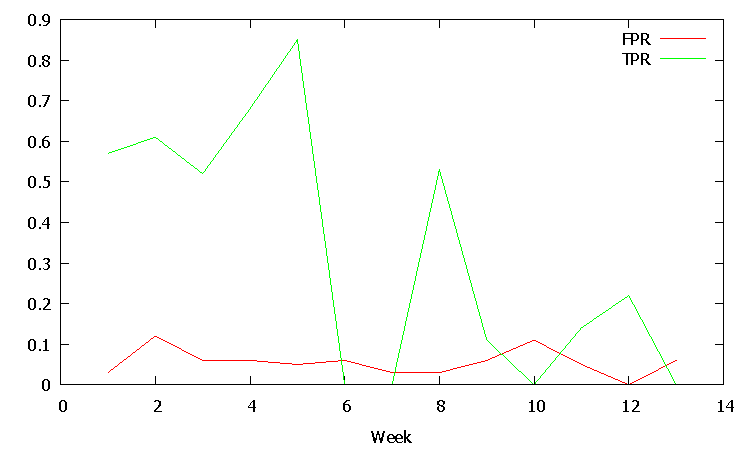
\includegraphics[scale=1.0]{images/voc_dtwknn_test.pdf}
\caption{Weekly \emph{TPR} and \emph{FPR} for DTW and kNN based model starting from the beginning of December 2012.}
\label{fig:voc_dtwknn_test}
\end{figure}
\end{center}

The \emph{FPR} is very small as it was in the parameter selection, too. The \emph{TPR} maintains its level at 0.50-0.60 for five weeks and then drops significantly. Looking at the data shows that the number of limit-exceeding peaks almost disappear in the wintertime. Thus, it is very difficult for the model to predict these rare events.

\subsection{Classification with Wavelets and SVMs}
\subsection*{Variable: CO2}
First, let us look at the product of the Haar Wavelet Transform. Figure~\ref{fig:wavelets} shows the original time series and Haar Wavelets with three different levels, 1, 2 and 10. The Weka Wavelet algorithm chooses the level from equation
\begin{align}
\mathbf{level} = \emph{ceil} \left ( \frac{\log{\emph{length}}}{\log{2}} \right ),
\end{align}
where \emph{length} is the length of the time series and \emph{ceil()} rounds the answer up to the nearest integer. When the length of the time series is about 1000 points, the equation gives 10 levels.


\begin{figure}[h!]
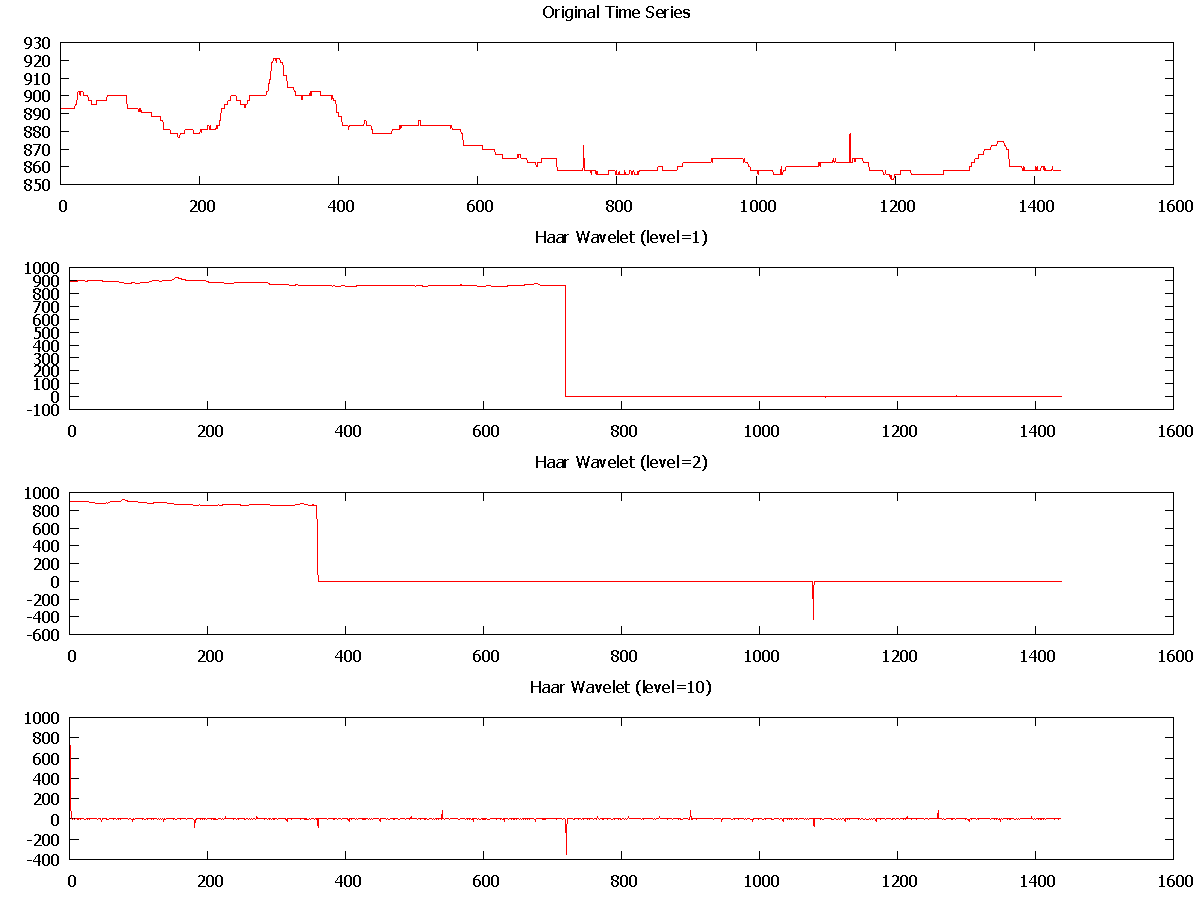
\includegraphics[scale=0.8]{images/wavelets.pdf}
\caption{Original time series and Haar Wavelets with three different levels, 1, 2 and 10.}
\label{fig:wavelets}
\end{figure}


This time the model parameters, $\gamma$ and \emph{C} should have a major impact on the classification results. Hence, we will perform an actual cross validation with 5 folds as described in Chapter 3.6.1. The data used is again from November 2012 so the resulting classifier can be compared to the one in the previous chapter.

For each parameter combination a cross validation is performed. Then, an average $AC_d$ from Equation~\ref{eq:acd} is calculated for each parameter combination. The best parameter combination is then used for training the model.

For parameter $\gamma$ the grid values are calculated using the Jaakkola Heuristics described in Equation~\ref{eq:svm_gamma} with $a_0$ set to five. This results in 11 different values for $\gamma$. For parameter \emph{C} we use a logarithmic grid $\{ 10^{i} \}$, $i = -2, ... 6$ to first find out the correct magnitude for \emph{C}.

The average accuracies and calculated $AC_d$s for \emph{C} and $\gamma$ are shown in Figures~\ref{fig:co2_svm_c} and \ref{fig:co2_svm_gamma}. Each point in the graphs is an average value of all the test runs with the given parameter value. There were a total of 55 runs for each value of \emph{C} and 45 runs for each value of $\gamma$.

\begin{center}
\begin{figure}[h!]
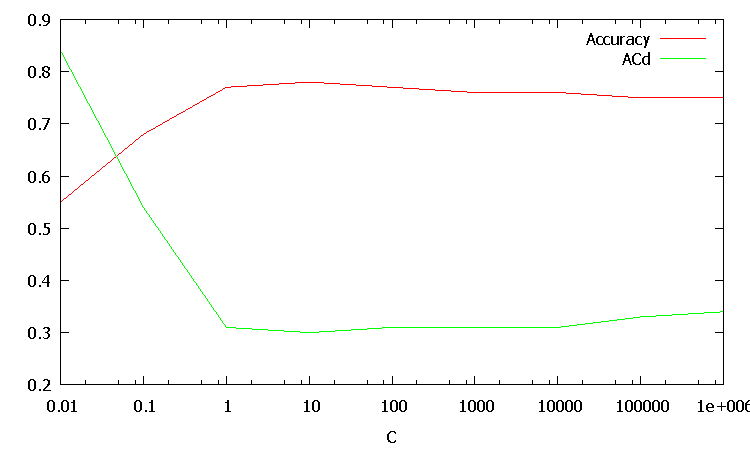
\includegraphics[scale=1.0]{images/co2_svm_c.pdf}
\caption{SVM classifier performance as a function of \emph{C}.}
\label{fig:co2_svm_c}
\end{figure}
\end{center}

\begin{center}
\begin{figure}[h!]
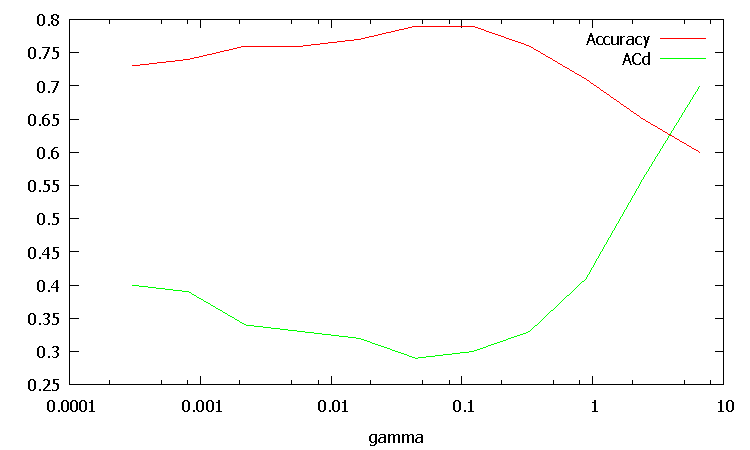
\includegraphics[scale=1.0]{images/co2_svm_gamma.pdf}
\caption{SVM classifier performance as a function of $\gamma$.}
\label{fig:co2_svm_gamma}
\end{figure}
\end{center}

The average classifier performance improves as \emph{C} increases to one. After that the accuracy decreases slowly. As the parameters might not be independent of each other, these graphs alone can not be used to select the optimal values. Figure~\ref{fig:co2_svm} shows accuracy as a function of both \emph{C} and $\gamma$. By inspecting the graphs a suitable combination for the parameters could be $C = 10$ and $\gamma = 0.05$. 

\begin{center}
\begin{figure}[h!]
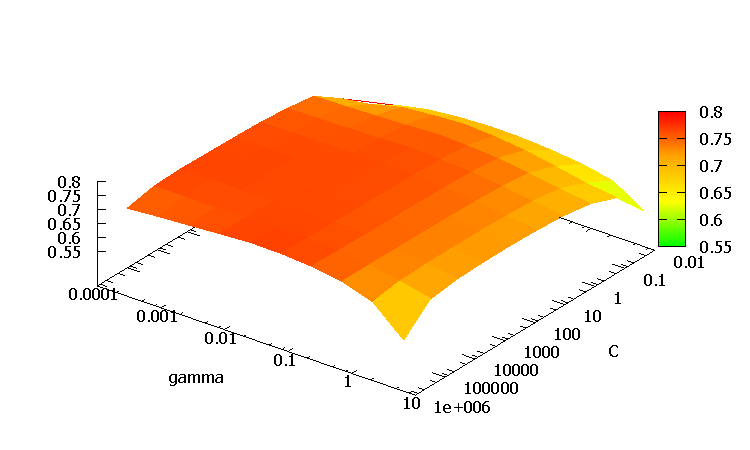
\includegraphics[scale=1.0]{images/co2_svm.pdf}
\caption{SVM classifier accuracy as a function of \emph{C} and $\gamma$.}
\label{fig:co2_svm}
\end{figure}
\end{center}

Next, the Wavelet and SVM model is trained with 14 days of data. This can not be done, however, with the same data we used for parameter selection because that approach would end up with overfitting. The values for \emph{TPR}, \emph{FPR} and Accuracy are shown in Figure~\ref{fig:co2_waveletsvm_test}.

The figure shows that the performance of this classifier varies much more than that of the DTW and kNN model.

\begin{center}
\begin{figure}[h!]
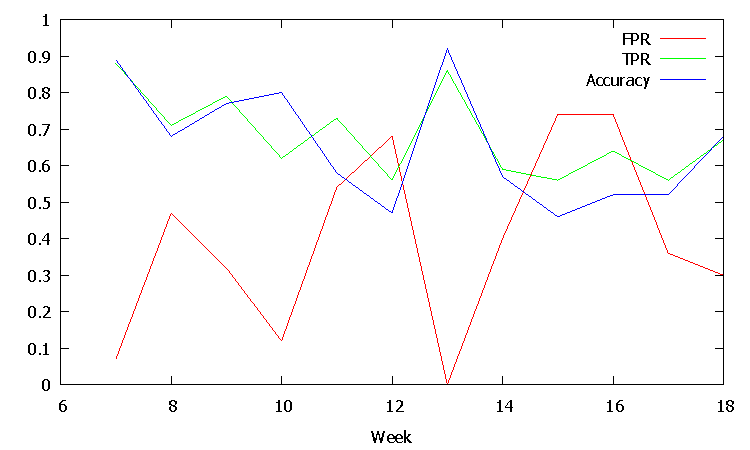
\includegraphics[scale=1.0]{images/co2_waveletsvm_test.pdf}
\caption{Wavelet and SVM based model performance with $C = 10$ and $\gamma = 0.05$.}
\label{fig:co2_waveletsvm_test}
\end{figure}
\end{center}



%\subsubsection*{Variable: VOC}
%We use the same data as for DTW and kNN based model in the %last section. Again, a grid search for optimal parameter %values is performed with data from November 2012. Since it %was shown with DTW and kNN model that the 

\section{Computational Performance}
Standard DTW algorithm has time complexity of $\mathcal{O}(N^2)$, where \emph{N} is the length of the time series. However, the FastDTW library we are using promises time complexity of $\mathcal{O} (N)$ \cite{salvador04}. The training phase of DTW and kNN is $\mathcal{O}(1)$ operation and takes only a few milliseconds because no calculations are performed. The given training set is simply saved into the model. Only when a new instance is classifier, DTW algorithm is run against each training sample and then \emph{k} closest are selected for voting.

\begin{center}
\begin{figure}[h!]
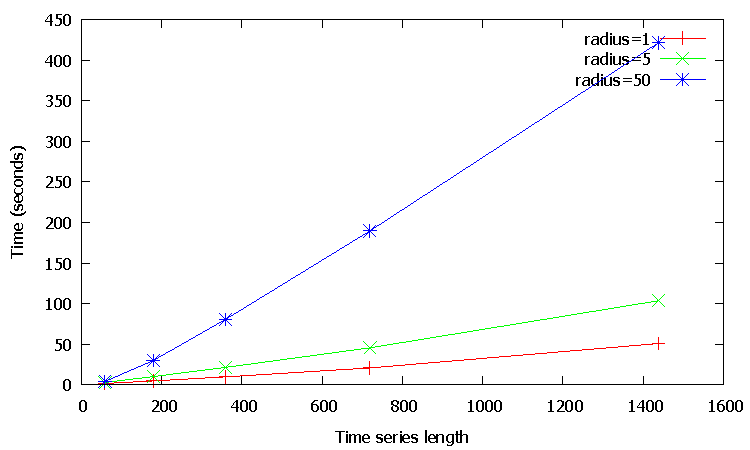
\includegraphics[scale=0.7]{images/dtw_knn_performance_timeseries_length.pdf}
\caption{DTW and kNN based model's performance as a function of time series length.}
\label{fig:dtw_knn_performance_timeseries_length}
\end{figure}
\end{center}

Figure~\ref{fig:dtw_knn_performance_timeseries_length} shows the training time as a function of time series length. Different time series lengths were acquired by varying the \emph{windowLength} parameter from 10 minutes to 4 hours. The smaller the \emph{radius} parameter is, the shorter the calculation time is as the algorithm is stopped earlier. As the authors of FastDTW promised, the time complexity is linear for relatively small time series ($< 2000$ data points). For longer time series it soon becomes second-degree polynomial. \cite{salvador04}




The LibSVM promises time complexity of $\mathcal{O}(l)$, where $l$ is the length of the time series if no kernel evaluations are required and $\mathcal{O}(nl)$ when $n$ kernel evaluations are required \cite{libsvm}. To put it briefly, the SVM training should be linear. 

\begin{center}
\begin{figure}[h!]
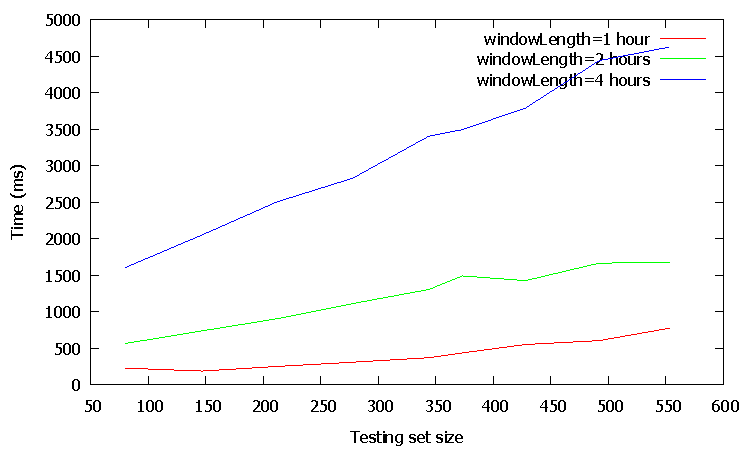
\includegraphics[scale=0.7]{images/wavelet_svm_performance.pdf}
\caption{Wavelet and SVM based model's performance as a function of training set size.}
\label{fig:wavelet_svm_performance}
\end{figure}
\end{center}

Figure~\ref{fig:wavelet_svm_performance} shows the testing time of Wavelet and SVM based model when the training set size is held constant at 139 data points. Clearly, increasing the number of test instances increases the execution time linearly. This same applies for DTW and kNN based model. 

If the number of test instances is also increased, the time complexity of DTW and kNN based model is no longer linear but rather follows a polynomial relationship, possibly a second-degree one. This is because each extra testing instance must be evaluated against each extra training set instance. The exact form of this polynomial could be found by regression analysis.

Wavelet and SVM based model, on the other hand, remains at linear computational time despite the increased number of both training and testing samples. This follows from the linear time requirements of both discrete Haar transform and  

\section{Discussion}
The biggest difference between the two models was the computational time needed to train and test the models. DTW and kNN based model takes about few minutes while with Wavelet and SVM based model only a few seconds are enough. 

Even though the FastDTW algorithm uses various methods, such as data abstraction and warping path constraints, to speed up the calculations, it still is a relatively slow algorithm. There is no way to decrease the number of DTW calculations as each testing instance must be evaluated against each training instance.

Calculating the Discrete Haar Wavelet Transform for small time series is not computationally demanding. It only consists of a series of addition and subtraction operations until the desired level is achieved. Weka Wavelet library doesn't provide any method to manually set to level up to which the transformation is performed. It would be useful to evaluate the classifier performance as a function level used for Haar Transform.

The core of LibSVM is written in C programming language which achieves better performance than if it was written in pure Java. LibSVM uses two techniques, shrinking and caching, to decrease the iteration time \cite{libsvm}. The shrinking method identifies and removes some bounded elements resulting in a smaller optimization problem. The quite advanced mathematics behind this method are not review here. The caching method stores kernel evaluations into memory for later use and thus avoids recalculations.

When it comes to classification performance, it was shown that regular peaks are much more predictable than ones that occur relatively rarely. With $CO_2$ the DTW and kNN based model achieved an acceptable performance with accuracy being over $80 \%$, True Positive Rate (TPR) over $75 \%$ and False Positive Rate (FPR) under $10 \%$. 

When comparing a model that was trained once to a model that was trained with regular intervals, no differences were found. The reason for these findings might be that the signal was close to a stationary process whose mean and variance remained about the same for the whole testing period. It was also shown that the installation of mechanical ventilation system changed the indoor air conditions dramatically and the performance of the classifier plummeted.

With VOC variable it was shown that the system's time parameters have a major impact on the performance. For example, the optimal choice of \emph{windowLength} parameter may increase the accuracy from about $60 \%$ to over $75 \%$. The number of indoor air particles decreased in the winter and the classifier failed heavily after that.


The Wavelet and SVM based model is difficult to tune. In addition to system's time parameters, it has two parameters, \emph{C} and $\gamma$ that derive from the mathematical equations. With $CO_2$ it was shown that both these parameters have optimal values that maximize the accuracy and minimize the $AC_d$. However, the testing accuracy varied a lot compared to the first model. LibSVM provides additional parameters, such as $\epsilon$ for stopping the iteration and weight parameters for different classes, that are sure to affect the observed performance but were not investigated here.

The second model is much more sensitive to the available data. Even small changes in the time parameters transformed the classifier from a nearly perfect one to a completely useless one. Especially with VOC, which has sharp peaks occurring rarely, this model lacks some kind of dynamic time parameter tuning that would optimize the length and the difference of the time windows on the go.

All in all, the results were quite close to my expectations. The easy-to-use DTW and kNN based model outperformed the more sophisticated Wavelet and SVM based model. The latter model, however, showed potential for predicting regular peaks in less time then the first model. With a little bit more parameter tuning I am pretty confident that Haar Wavelets and SVMs can work together with reasonable results.




\clearpage

\chapter{Conclusions} 

The goal of this thesis was to develop a framework for predictive complex event processing. By combining CEP and Predictive Analytics (PA) the capabilities of CEP for pattern detection can be taken a step further towards a real-time alarm system. Building this kind of system consists of the following phases
\begin{enumerate}
\item{Setting up the sensors}
\item{Enabling data flow into the CEP engine}
\item{Identifying the phenomena and describing them with EPL clauses}
\item{Building and configuring the predictive component to receive alarms}
\item{Taking necessary actions}
\end{enumerate}

The first phase, setting up the sensors, requires either setting up physical sensors or simulating ones with a computer software. Since there were data available from a real-life case, it was a easy choice to ask for a permission to use it. This choice, nevertheless, came with a potential risk of the data being uninteresting or too complicated. The two sensors, $CO_2$ and VOC were chosen for testing because of their large value range. The consumption variables, such as electricity and heating, had to be left out because their values were in pulses and not in their actual units. This conversion would have caused too much extra work.

The second phase, the data flow from the sensors into the CEP engine can be further divided into two phases: a data flow from the sensors into our predictive framework and a data flow inside our predictive framework. The former begins with wireless sensors emitting measurements to a server via a router. The latter consists of downloading the data from the server and formatting them to Java objects that can be inserted into the CEP engine.

At the core of the predictive framework is to Esper CEP engine which, as a state-of-the-art open-source solution, is gaining more and more popularity among CEP developers. In this thesis only a small fraction of Esper's capabilities were used. Only relatively simple EPLs with some temporal logic and timers were used. More advanced features, such as context-dependent reasoning and direct database connections, could be used to extend the predictive framework into a more comprehensive house automation software.

The third phase, writing the EPL clauses, requires domain experts to define meaningful complex events. Since I do not have enough experience in environmental issues, a very simple complex event type was chosen. Detecting a variable exceeding a certain limit is, however, an important one according to the Finnish Indoor Society. By their definition, the indoor air quality is solely determined by a set of limits for different variables. \cite{sisailmaluokitus08}

The next step from our ``simple complex events'' would be to detect and predict a combination of variables exceeding a limit. This would give a more comprehensive image of the living conditions. Then, additional independent variables, such as weekday and season, could be used to add cycle detection to the platform. 

The fourth phase is the main focus point of this thesis. The predictive component is a separate CEP network that listens to the original network's inputs (measurements) and outputs (complex events) \cite{Fulop12}. The novel idea of this thesis was to construct the predictors and their labels with CEP. All the previous work done in this area builds the training and testing set manually, or at least they have no mentions of using CEP for that.

The fifth phase requires domain expertise to define the necessary actions. When it comes to limit exceeding complex events that we are investigating in this thesis, a possible action could be opening a window. Other actions include adjusting heating, cooling or ventilation. In case of an emergency situation, such as rising carbon monoxide levels, a loud alarm should be played in order to alert the residents. Since this system is already connected to the outside world, also the authorities could be notified and called automatically in that case.

Taking necessary actions is closely tied with the time parameters in our predictive framework. The time parameters, \emph{waitingTime} and \emph{eventTime}, define the prediction horizon that begins with a warning interval. The warning interval corresponds to the time needed to prevent the complex event from happening. Should a single topic be chosen for additional research, it would definitely be a more  thorough choice of time parameters.

This thesis has two different intersections with real-life applications. First, the motivation for this work stems from the MMEA research project which aims at creating a platform for environmental data exchange. The platform offers interfaces for external applications that can make use of the real-time sensor data. The predictive complex event processing platform that was developed in this thesis could be one of these applications.

Second, this thesis uses test data from ASTEKA project which builds intelligent houses that adapt to changing living conditions. Even though the real-life data is with no doubt very challenging to start with, the framework developed in this thesis showed some potential allowing smooth data flow and some promising result. Actually, the most successful parts of this thesis are related to data handling and integrating all the components together. With relatively little code actual sensor data is used for prediction and alerts are shown to the user.

The problems that were faced during the experimental part were mainly related to the applied methods and the available testing data. First, the used models, especially the Wavelet and SVM based one, have a fairly large number of parameters that affect the performance. For this reason each section in the results chapter is built from different types of results. This approach shows a cross-section of what kind of results can be achieved and how they can be represented in a tabular or a visual form. The parameter optimization needs definitely more investigation before the platform can be said to actually work.

Second, the available testing data was actual data from an actual test house. In real-life the $CO_2$ concentration is not the most interesting variable when it comes to alerting the residents. However, a $CO_2$ sensor located in a small room without mechanical ventilation is sensitive enough to show a lot of regular variation which our platform managed to predict very well. When the mechanical ventilation was installed and the regular peaks disappeared, the performance of our model decreased significantly.

As hypothesized before, the simpler DTW and kNN based model performed better than the more complex Wavelet and SVM model. Our complex event type, a variable exceeding a limit, can be predicted by detecting the rise in that variable. DTW captures this kind of information better probably because it stretches the two time series being compared so that the rising parts are matched. Wavelet transform, on one hand, is able to detect this kind of patterns but, on the other hand, lacks translation invariance, which means that the two signals might not be similar if they are in different phases. There are some methods available to overcome this problem. \cite{struzik99}

As already mentioned before, possible focus points for future research are
\begin{itemize}
\item{Better evaluation of what kind of data and which variables can be predicted}
\item{Defining more meaningful complex event with domain experts}
\item{Optimizing model parameters more thoroughly}
\end{itemize}

All of these were investigated to some extent but better results would definitely be obtained by focusing more on these three points. In the light of these shortcomings it is fair to say that the predictive framework developed in this thesis is just a proof-of-concept and still quite far from a real-life application.





\clearpage

\addcontentsline{toc}{section}{References}
\bibliographystyle{amsplain}
\bibliography{bibliography}

\clearpage

%% Liitteet 


\end{document}


